\documentclass[pdftex,11pt,a4paper,twoside]{report}

\usepackage{pdf_course_profile}

%\title{Cours d'�lectricit�}

\title{\begin{flushright}
    \rule{15cm}{1mm}\\
    \vspace{8mm}
    \huge{\bf{Electricit�}}\\
    \rule{15cm}{1mm}\\
    \large{Cours du CNAM - CPDA 1�re ann�e - 2006/2007}\\
    \today\\
    \small{Version 0.3.2}\\
    \end{flushright}
}

\author{Guillaume Pellerin / Christophe Langrenne\\
	CNAM - Chaire d'Acoustique\\
    5, rue du Vertbois F-75003 Paris\\
    \emph{guillaume.pellerin@cnam.fr}
}

\begin{document}

\maketitle
\newpage

\input{elec_cpda_cnam-resume}
\newpage

\setcounter{page}{3}
\tableofcontents
\cleardoublepage
\renewcommand{\labelitemi}{$\bullet$}

%%%%%%%%%%%%%%%%%%%%%%%%%%%%

\chapter{Electrostatique}\label{chap_elecstat}
\input{elec_cpda_cnam-chap_elecrostatique}
\cleardoublepage

\chapter{Electrocin�tique}\label{chap_eleccine}

\section{Rappels}
\subsection{Mobilit� des charges~: courant �lectrique}

Soit deux conducteurs $A$ et $B$ isol�s en �quilibre avec $V_{A} > V_{B}$ (voir figure \ref{cond_charge}). $A$ poss�de en exc�s des charges positives et $B$ poss�de en exc�s des charges n�gatives.

\begin{figure}[h]
\begin{center}
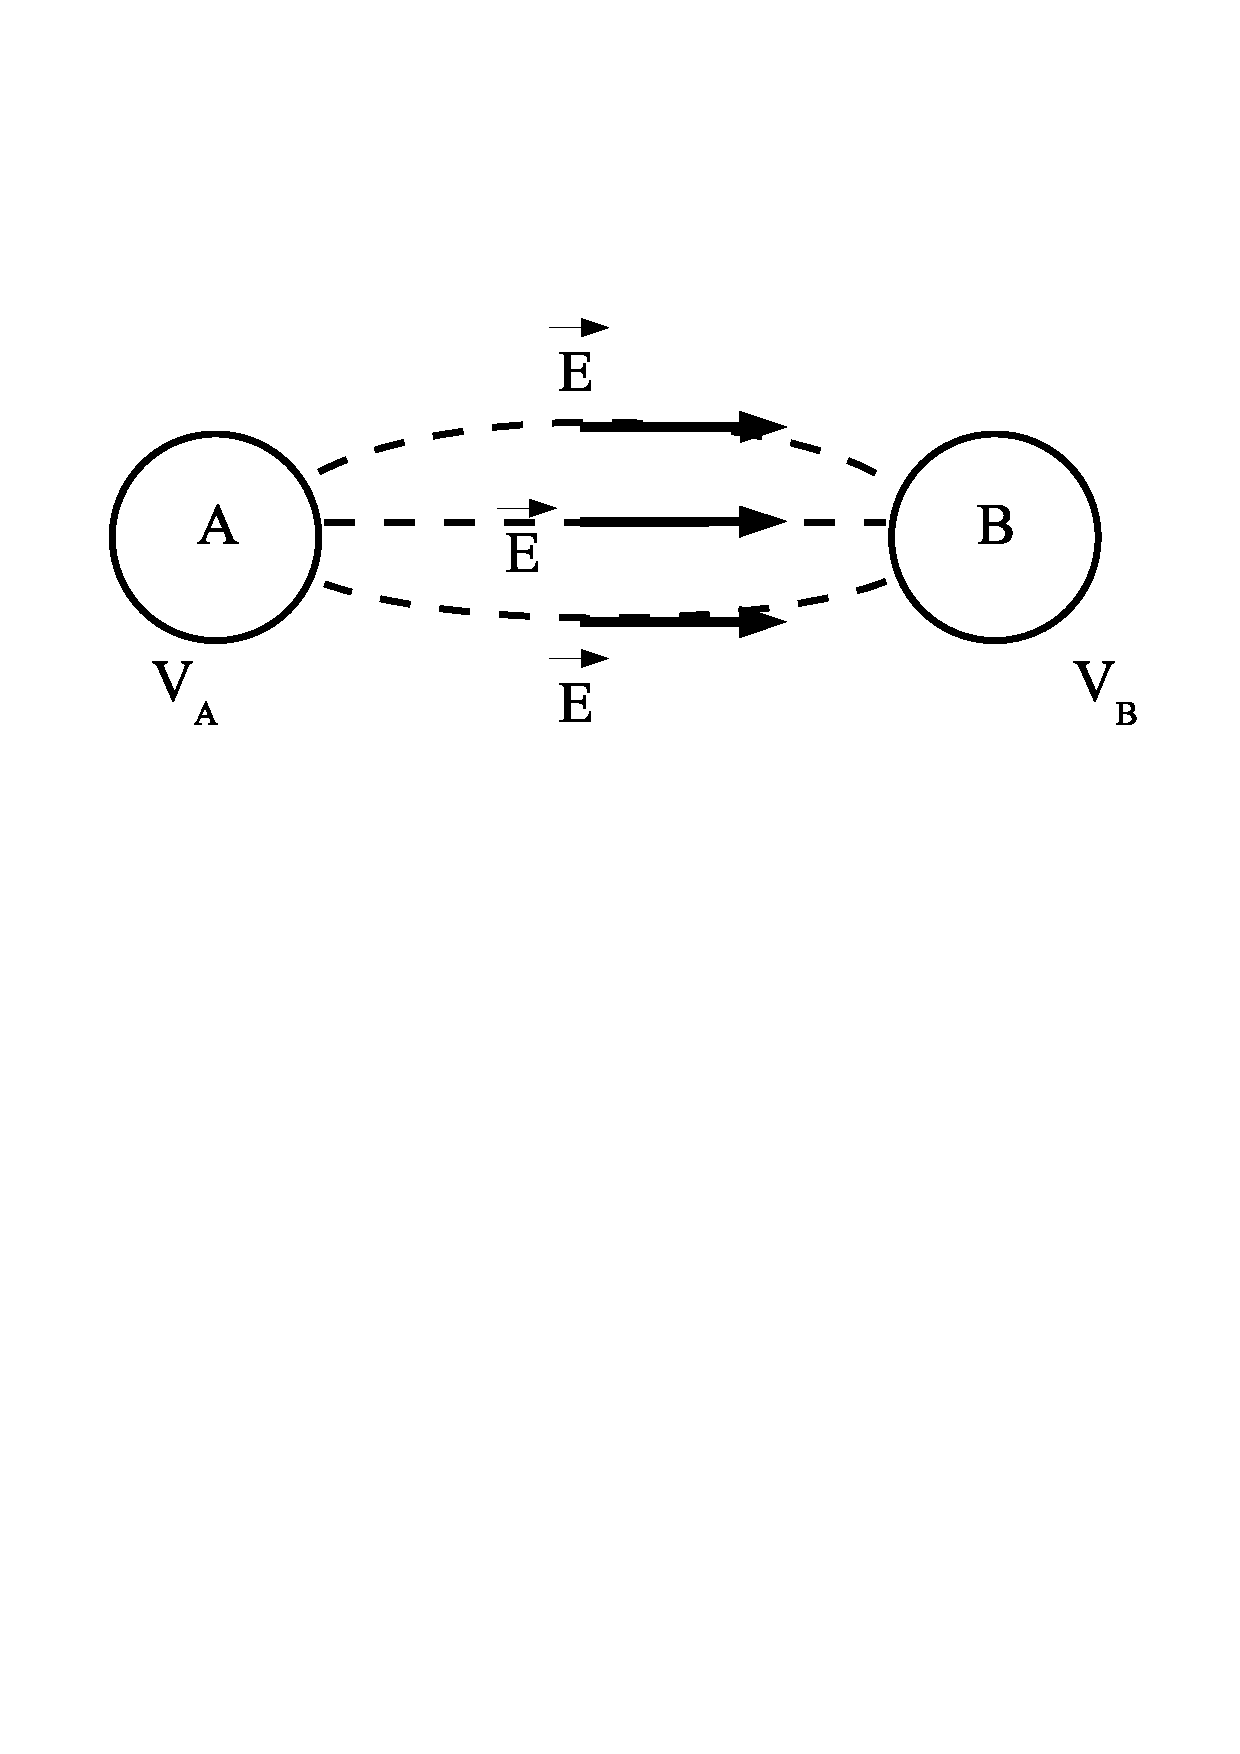
\includegraphics[clip=true,viewport=0cm 17cm 20cm 25cm,scale=0.38]{./figures/Conducteurs_charges.pdf}
\caption{Conducteurs charg�s isol�s en �quilibre.}\label{cond_charge}
\end{center}
\end{figure}

Si on relie les deux conducteurs par un fil �galement conducteur, il y a un transfert de charge pour que tout point soit au m�me potentiel. Ensuite, $A$ et $B$ sont au m�me potentiel, le champ �lectrique s'annule alors ainsi que le courant.

Le d�placement des �lectrons libres est quasiment instantan� (r�gime transitoire). Supposons que le pr�c�dent conducteur isol� $B$ soit un r�servoir d'�lectrons libres, c'est-�-dire que l'on arrive � maintenir son potentiel $V_{B}$. Si on fait en sorte que les �lectrons exc�dentaires du conducteur $A$ quittent le mat�riau pour maintenir le potentiel $V_{A}$, le champ �lectrique initial est r�tabli et le d�placement des �lectrons � l'int�rieur du fil conducteur est entretenu. Le champ $\vec{E}$ qui assure le d�placement des �lectrons et la circulation du courant est appel� \textbf{champ �lectromoteur}.

\subsection {Densit� de courant �lectrique}

\begin{figure}[h]
\begin{center}
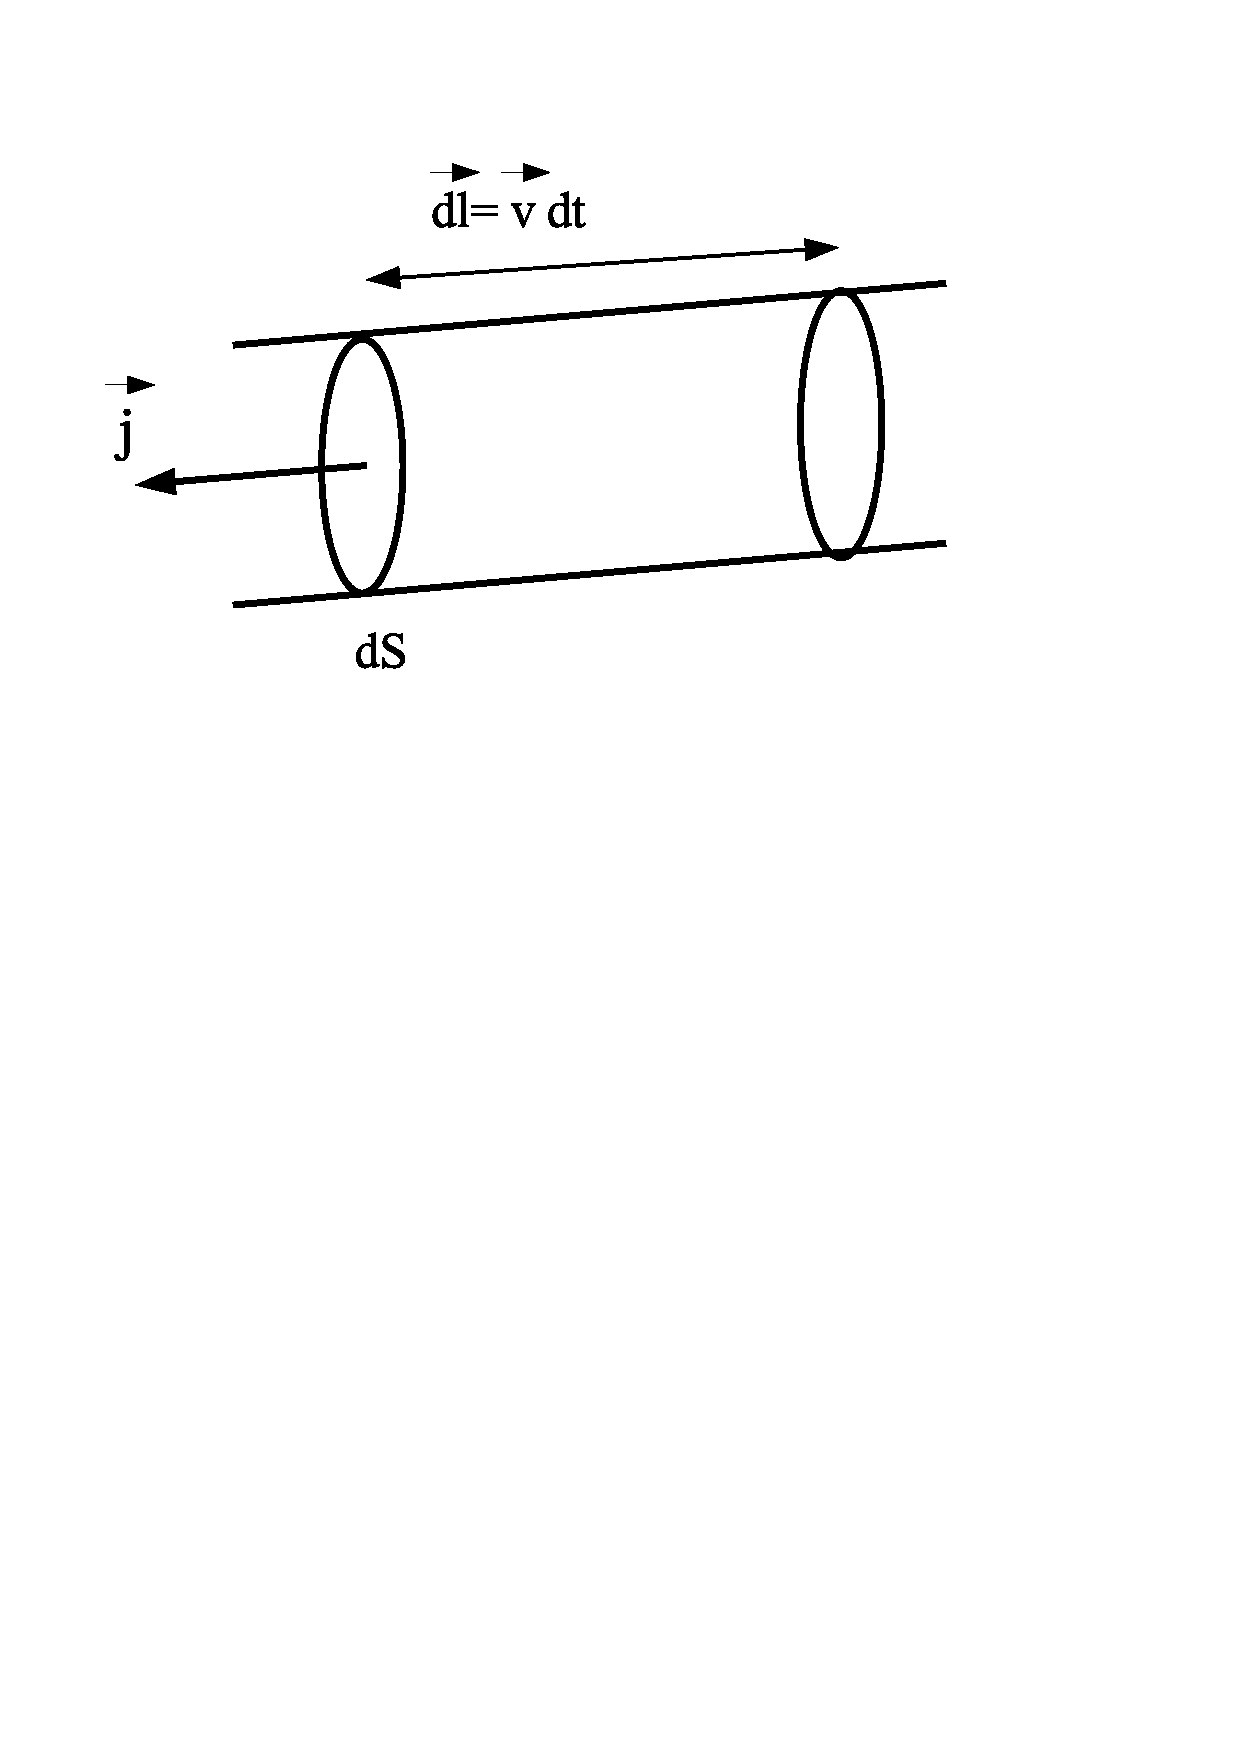
\includegraphics[clip=true,viewport=0cm 18cm 20cm 27cm,scale=0.38]{./figures/densite_de_courant.pdf}
\caption{Param�trisation d'un �l�ment de fil pour le calcul du courant.}\label{sch_cour}
\end{center}
\end{figure}

Le courant est produit par un d�placement organis� de charges, � une certaine vitesse. Consid�rons un fil conducteur de section $S$, dans lequel se trouve une densit� de charge volumique $\rho$, anim� d'une vitesse $\vec{v}$ (cf. figure \ref{sch_cour}). Pendant un instant $\ud t$, ces charges parcourent une distance $\vec{v} \ud t$. Soit $\vec{n} \ud S$ un �l�ment infinit�simal de surface mesur�e sur la section du fil, orient� dans une direction arbitraire. La quantit� de charge �lectrique qui traverse cette surface pendant $\ud t$ est celle contenue dans le volume �l�mentaire $\ud V$ associ� et s'�crit~:

$$\ud Q = \rho \ud V = \rho \vec{v} \ud t \cdot \vec{n} \ud S$$

On voit alors appara�tre un vecteur qui d�crit les caract�ristiques du milieu conducteur et qu'on appelle la \textbf{densit� de courant}~:

$$\vec{j} = \rho \vec{v}$$

exprim� en Amp�res par m�tre carr� ($\mathrm{A.m^{-2}}$).

Le courant $dI$ circulant dans la portion de fil est la charge traversant la section, et est reli� � la densit� tel que~:

$$\ud I = \frac{\ud Q}{\ud t}$$

On en d�duit :

$$I = \frac{1}{\ud t} \iint_{S} \ud Q = \frac{1}{\ud t} \iint_{S} \vec{j} \ud t \cdot \vec{n} \ud S$$

soit :

\begin{equation}
\boxed{I = \iint_{S} \vec{j} \cdot \vec{n} \ud S}
\end{equation}

On avait d�finit le flux du champ �lectrique~: $\Phi = \iint_{S} \vec{E} \cdot \vec{n} \ud S$. De m�me, $I$ est le flux de la densit� de courant � travers la section du fil. Le sens du courant est donn� par le sens du vecteur densit� de courant.

\begin{rem}[Convention]
On suppose que le courant est d� au mouvement des charges positives vers les charges n�gatives : sens du courant. En fait, ce sont les �lectrons libres qui se d�placent, mais on conserve la convention pour des raisons historiques.
\end{rem}


\subsection{Loi d'Ohm locale (ou microscopique)}

Dans la plupart des conducteurs, on observe une proportionnalit� entre le densit� de courant et le champ �lectrostatique local~:

\begin{equation}
\boxed{\vec{j}=\gamma \vec{E}},
\end{equation}

o� le c\oe fficient de proportionnalit� $\gamma $ est appel� la \textbf{conductivit� du milieu}. La conductivit� est une grandeur locale positive d�pendant uniquement des propri�t�s du mat�riau, elle s'exprime en Siemens par m�tre et est �gale � l'inverse de la r�sistivit� du milieu $\eta = 1/\gamma $. Par exemple, le cuivre poss�de une conductivit� $\gamma_{Cu} = 58.10^{6}\  \mathrm{S.m^{-1}}$, tandis que celle du verre (isolant) est $\gamma_{Cu} = 10^{-11}\ \mathrm{S.m^{-1}}$.

\subsection{R�sistance d'un conducteur. Loi d'Ohm}

Consid�rons maintenant une portion AB d'un conducteur parcouru par un courant $I$. S'il existe un courant $I = \iint_{S} \vec{j} \cdot \vec{n} \ud S$, cela signifie qu'il y a une chute de potentiel entre $A$ et $B$, $U=V_{A} - V_ {B}=\int_{A}^{B} \vec{E} \cdot \vec{\ud l}$. Il existe un scalaire $R$, caract�ristique du conducteur, tel que~:

\begin{equation}\label{resist_cond}
R = \frac{U}{I} = \frac {\int_{A}^{B} \vec{E} \cdot \vec{\ud l}}{\iint_{S} \vec{j} \cdot \vec{n} \ud S} =\frac {\int_{A}^{B} \vec{E} \cdot \vec{\ud l}}{\iint_{S} \gamma  \vec{E} \cdot \vec{n} \ud S},
\end{equation}

o� l'unit� est l'Ohm (symbole $\Omega$).

\begin{bex}[Fil cylindrique homog�ne]
Dans le cas simple d'un conducteur filiforme de section $S$ o�, sur une longueur $L$, le champ �lectrostatique est uniforme, on obtient le lien entre la r�sistance d'un conducteur (propri�t� macroscopique) et sa r�sistivit� (propri�t� microscopique) tel que :

\begin{equation}\label{resist_fil}
R = \frac{E L}{\gamma E S}=\eta \frac{L}{S}
\end{equation}

dont l'unit� est le $\Omega.m$ (Ohm m�tre).
\end{bex}


\subsection{Association de r�sistances}

\subsubsection{R�sistances en s�rie}

Soient $n$ r�sistances $R_{i}$ mises bout � bout dans un circuit et parcourues par un courant $I$. La tension aux bornes de la cha�ne s'�crit simplement~:

$$U = (V_{0} - V_{1}) + (V_{1} - V_{2}) + \cdots + (V_{n-1} - V_{n})=R_{1} I + R_{2} I+ \cdots + R_{n} I,$$

Le r�sistance totale est donc analogue � celle obtenue par une r�sistance unique dont la valeur est~:

\begin{equation}
\boxed{R = \sum_{i=1}^{n}R_{i}.}
\end{equation}

\subsubsection{R�sistances en parall�le}

Soient $n$ r�sistances $R_{i}$ branch�es en parall�le sous une tension $U = V_{1} - V_{2}$ et aliment�es par un courant $I$. Le courant se s�pare alors en $n$ courants~:

$$I_{i} = \frac{U}{R_{i}},$$

dans chacune des $n$ branches. Nous avons alors (propri�t� de conservation du courant)~:

$$I = \sum_{i=1}^{n} I_{i} = \sum_{i=1}^{n} \frac{U}{R_{i}} = \frac{U}{R},$$

c'est-�-dire que l'ensemble des $n$ branches est analogue � une r�sistance �quivalente en s�rie �gale � :

\begin{equation}
\boxed{\frac{1}{R} = \sum_{i=1}^{n} \frac{1}{R_{i}}}
\end{equation}


\section{El�ments d'un circuit �lectrique}

\subsection{Notion de circuit �lectrique}

\begin{defi} Un circuit �lectrique est constitu� d'un ensemble de dispositifs appel�s \textbf{dip�les}, reli�s entre eux par un fil conducteur et formant ainsi une structure ferm�e. Un \textbf{n\oe ud} d'un circuit est une interconnexion o� arrivent 3 fils ou plus. Une \textbf{branche} est un tron�on de circuit situ� entre deux n\oe uds. Enfin, une \textbf{maille} est un ensemble de branches formant une boucle ferm�e.
\end{defi}

Un \textbf{dip�le} s'ins�re dans un circuit par l'interm�diaire de deux p�les, l'un par o� s'effectue l'entr�e du courant (borne $+$), l'autre la sortie (borne $-$). Il est caract�ris� par sa r�ponse � une diff�rence de potentiel $U$ entre ses bornes~: c'est-�-dire la courbe caract�ristique $I=f(U)$ qui, pour un dip�le passif, passe par l'origine. Un dip�le actif fournit un courant (positif ou n�gatif) m�me en absence de tension. Enfin, on appelle dip�le lin�aire tout dip�le dont la courbe est une droite.

Nous avons vu que, dans tout conducteur, la pr�sence d'une r�sistivit� entra�ne une variation de tension entre 2 noeuds travers�s par le m�me courant. Les fils �lectriques reliant les dip�les imposent ainsi leurs r�sistances propres qui s'ajoutent � la r�sistance globale du circuit. Dans la majorit� des cas d'�lectronique de puissance, ces r�sistances internes sont faibles devant celles des dip�les. Les fils sont alors suppos�s �quipotentiels. Cette hypoth�se n'est par contre plus valable dans le cas de courants de faible intensit� (�lectronique fine, micro-processeurs, etc...).

\begin{rem}
Nous nous int�ressons ici � des cas o� le courant est �tabli de fa�on permanente dans le circuit. L'intensit� y est alors la m�me en tout point. Cela exige �videmment que le circuit soit \emph{ferm�}.
\end{rem}

\subsection{Puissance �lectrique disponible}

Soit une portion $AB$ d'un circuit, parcourue par un courant permanent $I$ allant de $A$ vers $B$. L'existence de ce courant implique que le potentiel en $A$ est sup�rieur � celui en $B$. Cette diff�rence de potentiel se traduit par l'existence d'un champ �lectrostatique $\vec{E}$ produisant une force de Coulomb $\vec{F} = q \vec{E}$ capable d'acc�l�rer une charge $q$. Ainsi, soit $P_{q} = \vec{v} \cdot \vec{E}$ la puissance n�cessaire pour communiquer une vitesse $\vec{v}$ � une particule de charge $q$ quelconque. Sachant que dans ce conducteur il y a $n$ porteurs de charge par unit� de volume, la puissance totale $P$ mise en jeu dans le brin $AB$ parcouru par un courant $I$ s'�crit~:

\begin{equation*}
\begin{split}
P & = \iiint_{brin AB} nP_{q}\ \ud V \\
& = \int_{A}^{B} \iint_{Section} (nq\vec{v} \cdot \vec{dS}) \vec{E} \cdot \vec{\ud l} \\
& = \int_{A}^{B} \vec{E} \cdot \vec{\ud l} \iint_{Section} \vec{j} \cdot \vec{\ud S} \\
& = I \int_{A}^{B} \vec{E} \cdot \vec{\ud l} = I [V(A) - V(B)].
\end{split}
\end{equation*}

On en d�duit:

\begin{equation}
\boxed{P = UI}
\end{equation}

o� $U = V(A) - V(B) >0$ puisque le courant s'�coule de $A$ vers $B$. Cette puissance est donc la puissance �lectrique disponible entre $A$ et $B$ du simple fait qu'il y circule un courant $I$.

Suivant la nature du dip�le plac� entre $A$ et $B$ (r�cepteur), l'�nergie �lectrique disponible sera convertie sous une forme ou une autre. Dans le cas simple o� entre $A$ et $B$ ne se trouve qu'une r�sistance $R$, la puissance disponible $P$ ne sert qu'� faire chauffer la r�sistance puisque $U = RI$. Cela se traduit par une dissipation d'�nergie sous forme de chaleur, appel�e effet Joule, et dont la puissance vaut~:

\begin{equation}\label{joule}
\boxed{P_{j}=RI^{2}.}
\end{equation}

Cette �nergie peut �tre �galement reconvertie en rayonnement (lampe), �nergie m�canique (moteur), chimique (bac � �lectrolyse).

\begin{rem} Cette puissance peut aussi �tre n�gative lorsque $U = V(A) - V(B) <0$. Le dip�le fournit alors de l'�nergie, c'est un g�n�rateur.
\end{rem}

\subsection{N�cessit� d'une force �lectromotrice ou f�m}

Si on applique le raisonnement pr�c�dent � un circuit ferm�, c'est-�-dire si l'on regarde la puissance totale fournie entre $A$ et $B$ par la force de Coulomb, on obtient~:

$$P=I[V(A)-V(A)]=0,$$

c'est-�-dire une puissance nulle. Cela signifie qu'il ne peut y avoir de courant en r�gime permanent. Lorsqu'il y a un courant, cela implique que la force de Coulomb n'est pas responsable du mouvement global des porteurs de charge dans un conducteur.

\begin{rem}[Analogie]
Le courant dans un conducteur peut �tre compris avec l'analogie de la rivi�re circulant dans son lit. Pour qu'il y ait un �coulement, il faut que l'eau s'�coule d'une r�gion plus �lev�e vers une r�gion plus basse. Ainsi, le mouvement de l'eau d'un point �lev� vers un point plus bas est bien d� � la simple force de gravitation. Mais si l'on veut constituer un circuit ferm�, alors il faut fournir de l'�nergie (gr�ce � une pompe) pour amener l'eau � une plus grande hauteur, et le cycle peut alors effectivement recommencer.
\end{rem}

C'est exactement ce qui se passe dans un circuit �lectrique : une force autre que la force �lectrostatique doit permettre aux porteurs de charge de remonterle potentiel.

\begin{figure}[h]
\begin{center}
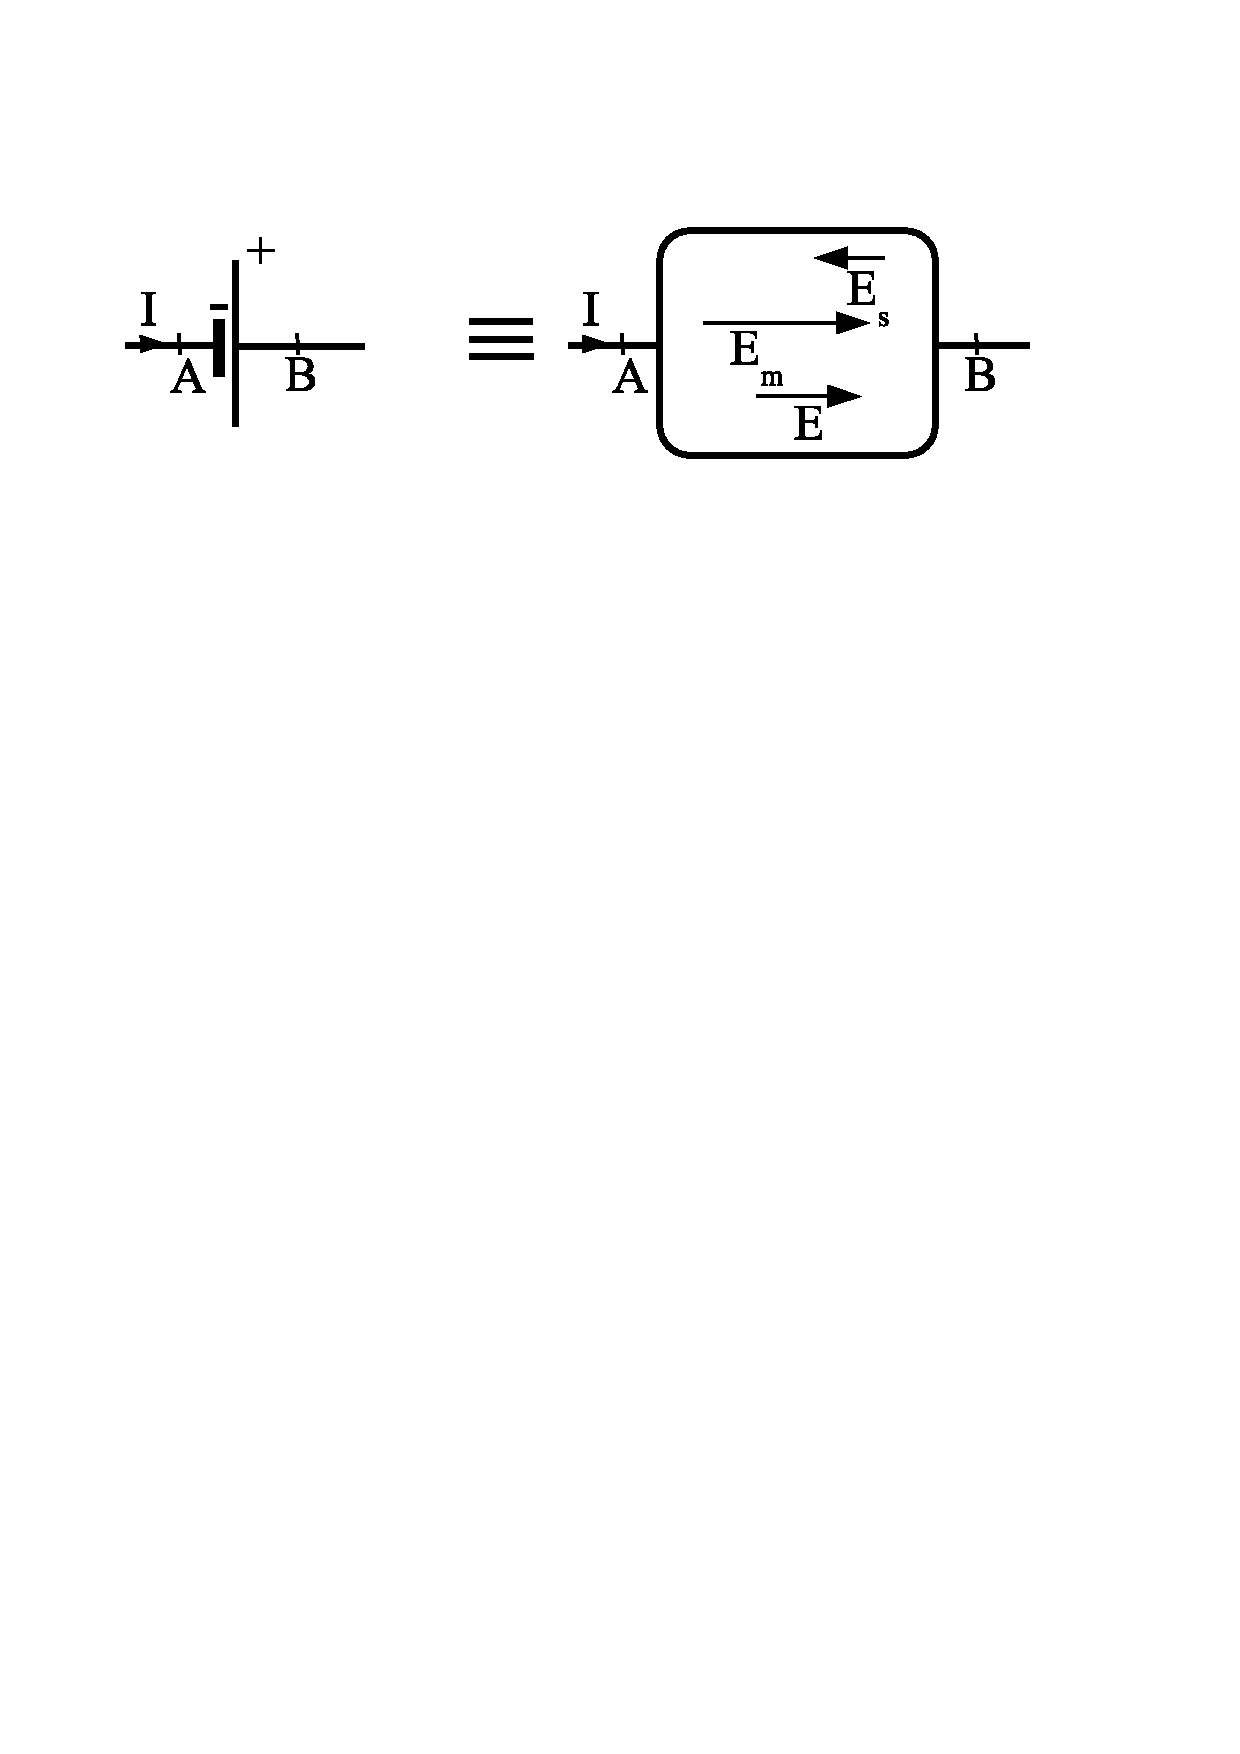
\includegraphics[clip=true,viewport=0cm 22cm 19cm 27cm,scale=0.55]{./figures/generateur.pdf}
\caption{Force responsable du courant.}
\end{center}
\end{figure}

La seule fa�on d'obtenir un r�gime stationnaire avec un courant permanent $I$, c'est donc d'avoir un champ suppl�mentaire, appel� champ �lectromoteur $\vec{E_{m}}$, sup�rieur en norme et dirig� en sens inverse de $\vec{E_{s}}$ (le champ �lectrostatique). Mettons maintenant le g�n�rateur en circuit ouvert ($I=0$). Le fait qu'une diff�rence de potentiel (ddp) se maintienne entre ses bornes implique n�cessairement la pr�sence d'une autre force compensant l'attraction coulombienne. Ainsi, � l'�quilibre et en l'absence de courant, on doit donc avoir $\vec{E_{s}} + \vec{E_{m}}=0$. Cela signifie donc que la ddp ou tension aux bornes d'un g�n�rateur ouvert vaut~:

$$V_{A}-V_{B}=\int_{A}^{B} \vec{E_{s}} \cdot \vec{\ud l}=-\int_{A}^{B} \vec{E_{m}} \cdot \vec{\ud l},$$

o�, bien �videmment, $V_{A}-V_{B}<0$. On appelle~:

$$e=\int_{A}^{B} \vec{E_{m}} \cdot \vec{\ud l}$$

\textbf{la force �lectromotrice} ou \textbf{f�m} du g�n�rateur ($e>0$ est exprim� en volts).

\subsection{Conventions}

Dans une branche, le sens du courant peut �tre choisi arbitrairement. L'orientation de la tension est ind�pendante du choix de l'orientation de l'intensit�~: $U_{AB}=V_A -V_B$ (de B vers A).\\

\begin{itemize}
\item Convention g�n�rateur~: $U$ et $I$ sont dans le m�me sens.
\item Convention r�cepteur~: $U$ et $I$ sont de sens contraire.\\
\end{itemize}

Si une branche contient un dip�le polaris� de f�m $e$, celui-ci sera compt� $+e$ si en parcourant la branche, on entre par la borne $-$ (au sens d'une chute de potentiel).

Exemple~:

\begin{figure}[h]
\begin{center}
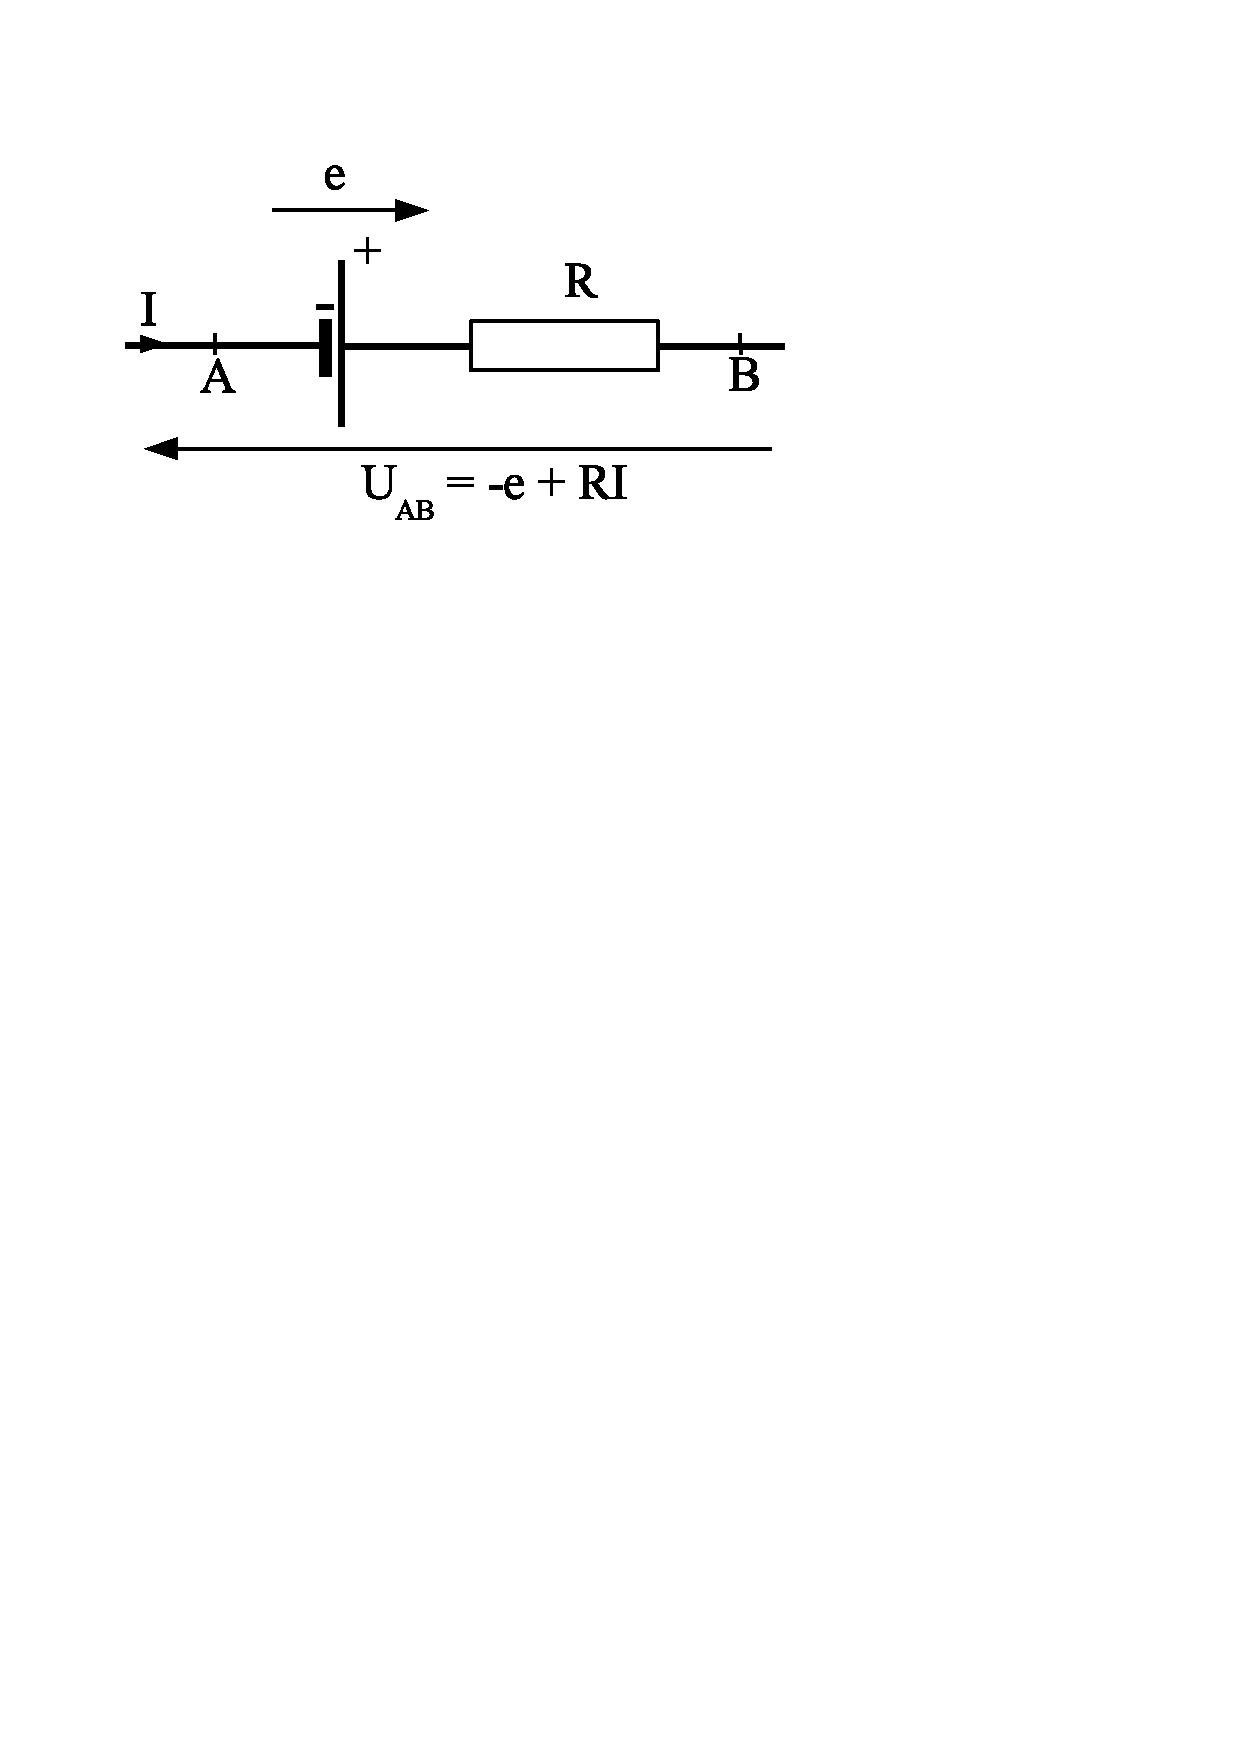
\includegraphics[clip=true,viewport=0cm 20.5cm 15cm 27cm,scale=0.65]{./figures/Calcul_de_tension.pdf}
\caption{Calcul de tension (exemple).}
\end{center}
\end{figure}

\subsection{Relation courant / tension}

Les dip�les sont caract�ris�s par une relation $U=f(I)$ ou $I=f(U)$ reliant la tension $U$ � leurs bornes au courant $I$ les traversant. Cette relation d�pend des dip�les. La repr�sentation graphique de cette relation s'appelle caract�ristique. Si cette caract�ristique passe par l'origine, le dip�le est dit passif ; dans le cas contraire, il est dit actif.

\begin{figure}[h]
\begin{center}
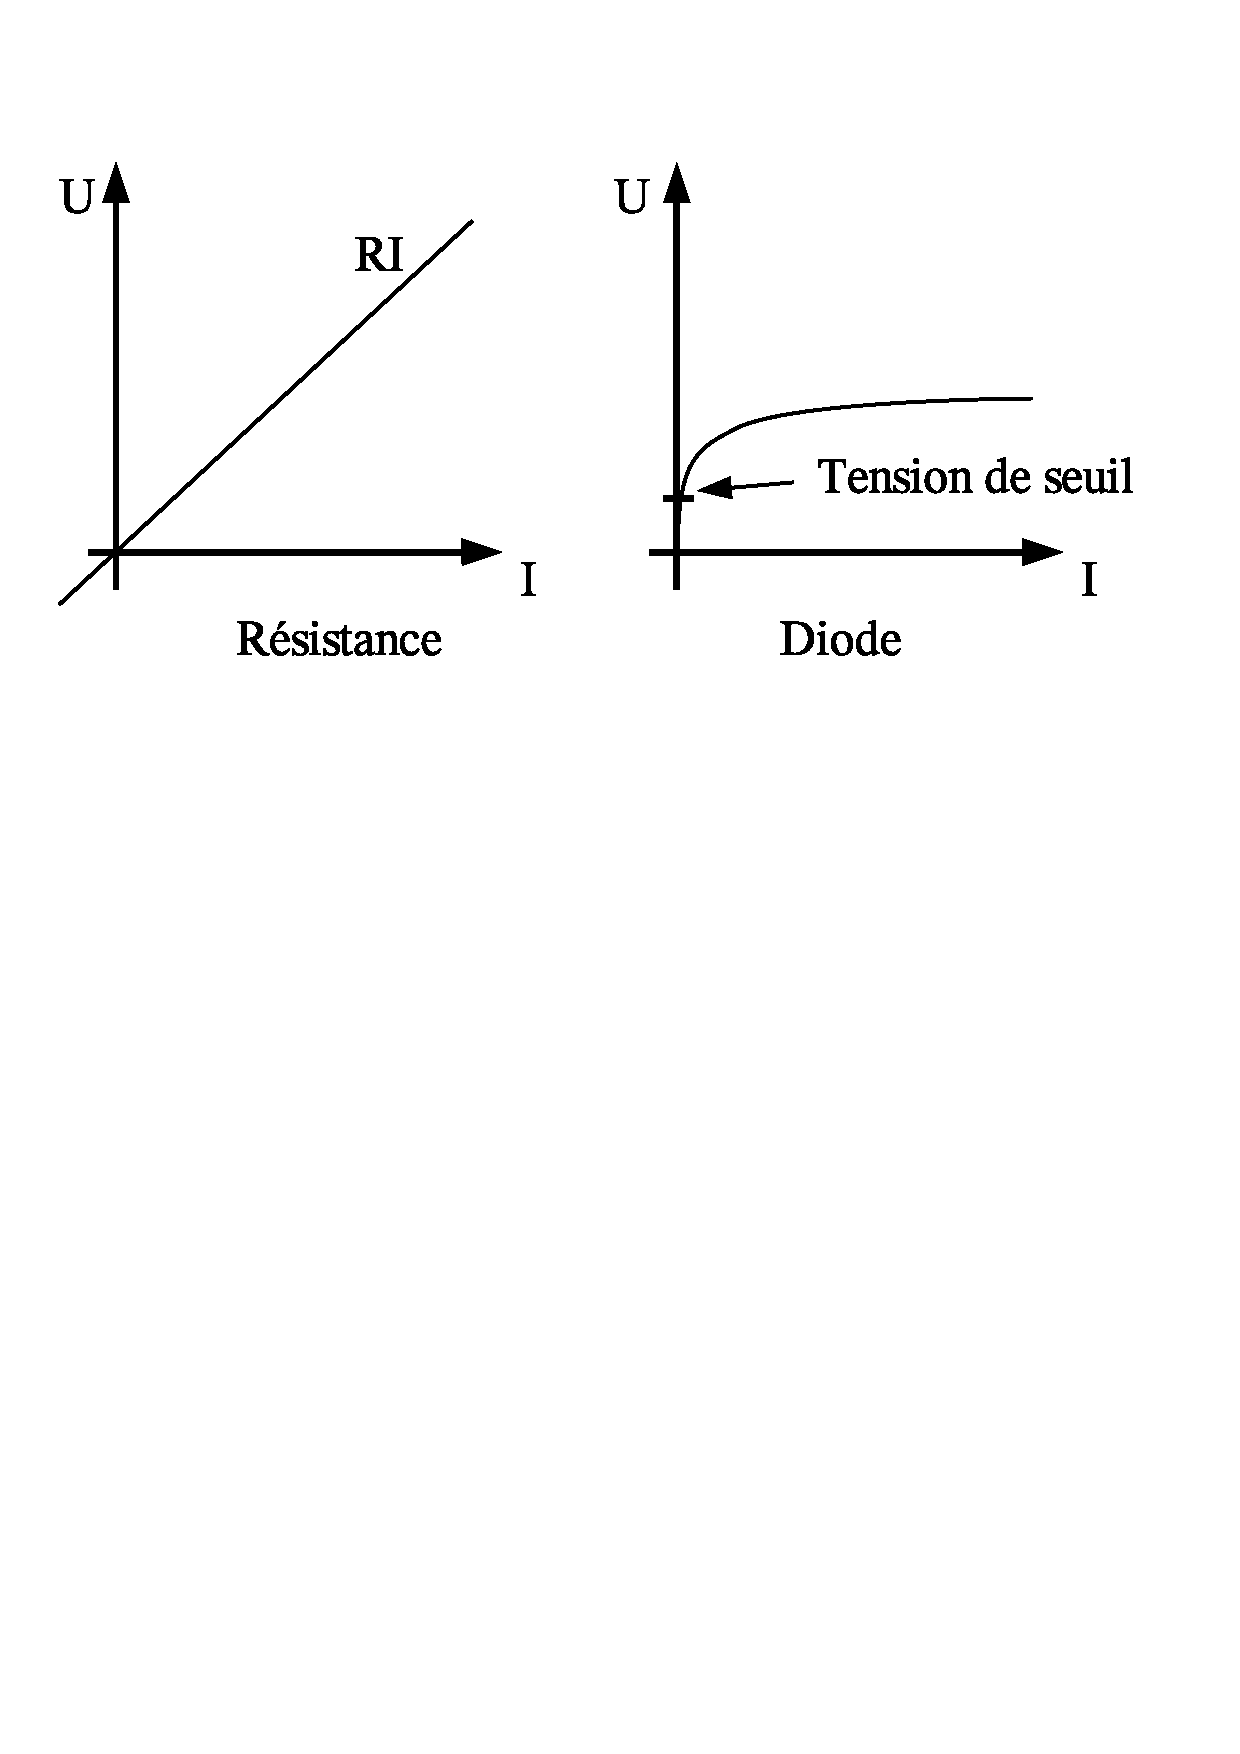
\includegraphics[clip=true,viewport=0cm 18cm 21cm 27cm,scale=0.75]{./figures/caracteristiques.pdf}
\caption{Exemples de caract�ristiques.}
\end{center}
\end{figure}

\subsubsection{Point de fonctionnement}

\begin{figure}[h]
\begin{center}
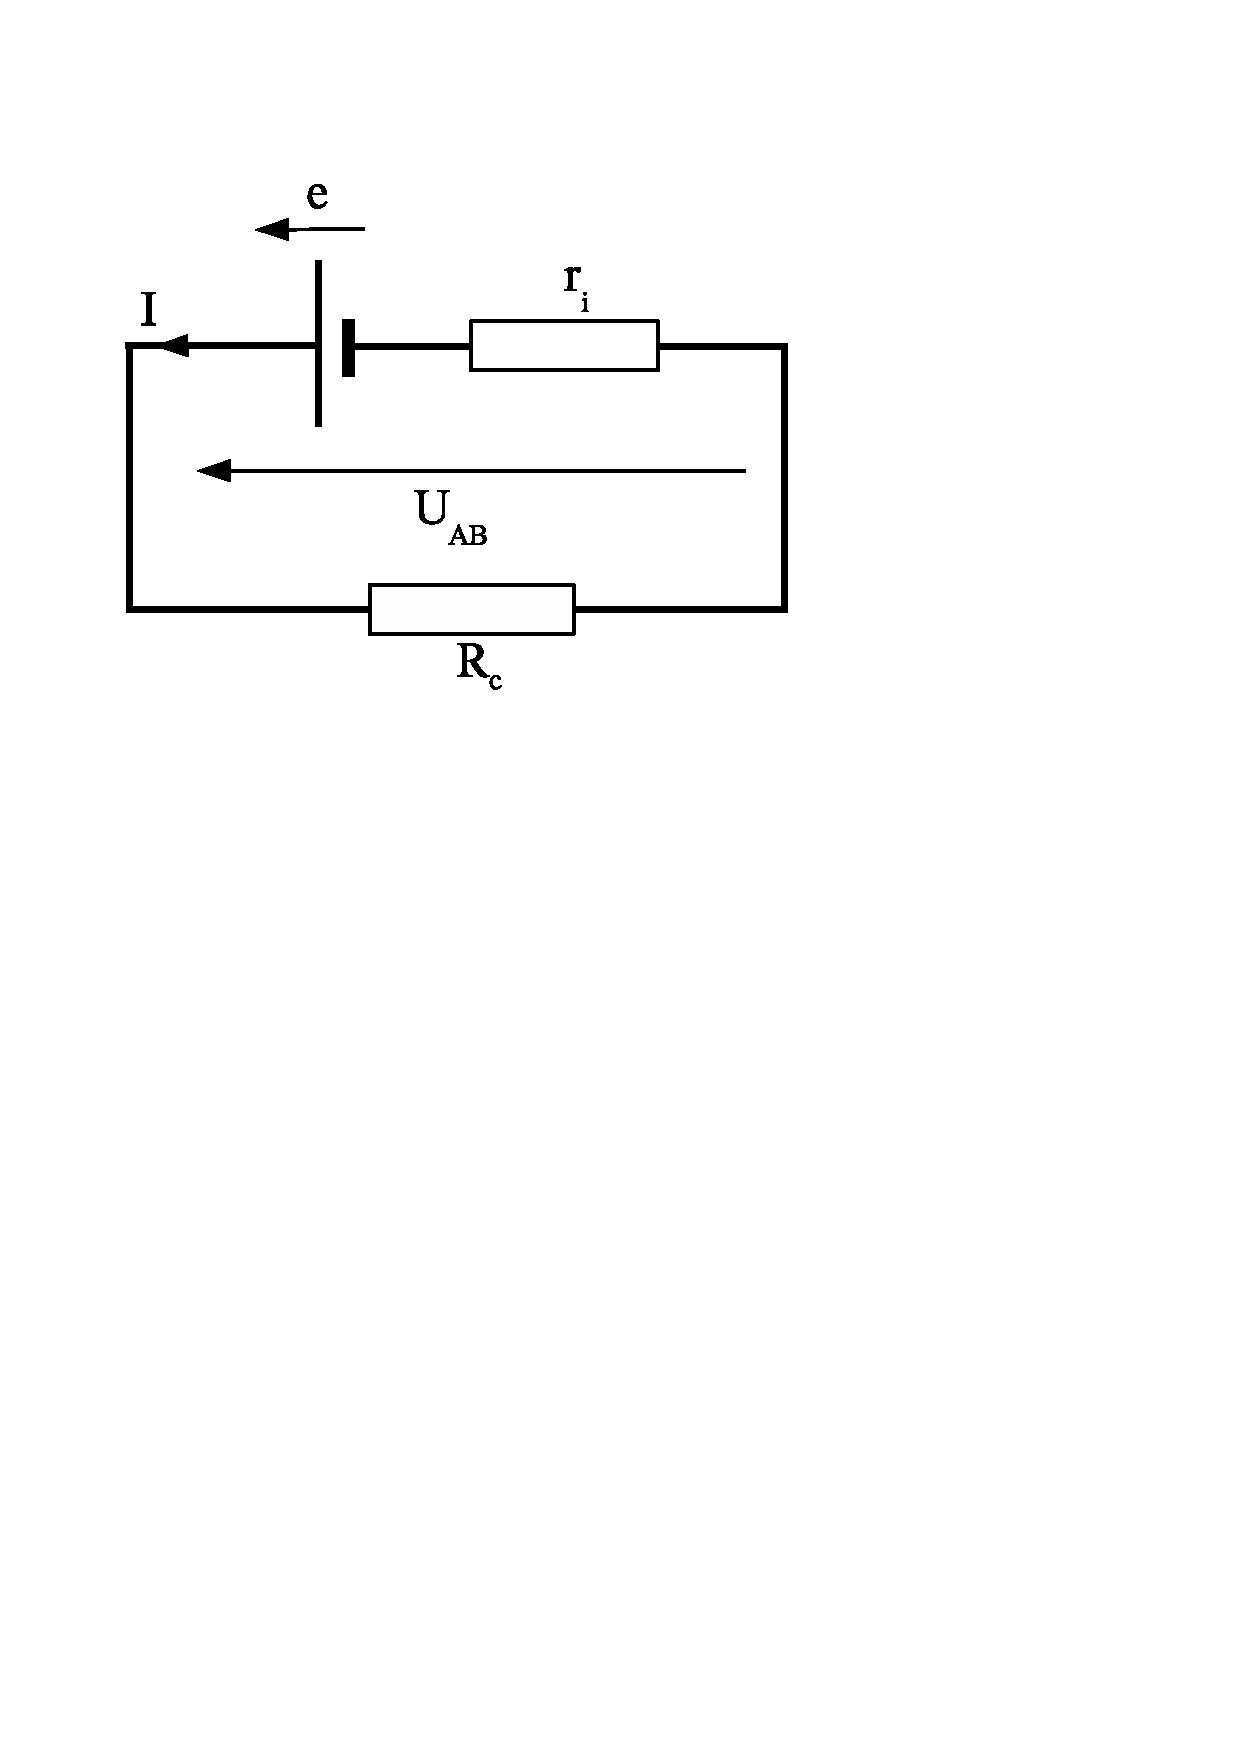
\includegraphics[clip=true,viewport=0cm 18cm 16cm 27cm,scale=0.5]{./figures/circuit.pdf}
\caption{Circuit �lectrique charg�}\label{circuit_01}
\end{center}
\end{figure}

Soit le circuit �lectrique donn� � la figure \ref{circuit_01}. Le courant s'�crit~:

$$I=\frac{e}{r_{i}+R_{c}}$$

d'o�

$$U_{AB}=e-r_{i}I=e-\frac{r_{i}e}{r_{i}+R_{c}}=\frac{e}{1+\frac{r_{i}}{R_{c}}}$$

Le \textbf{point de fonctionnement} est l'intersection des courbes $U_{AB}=e-r_{i}I=R_{c}I$ comme le montre la figure \ref{fig_pdf}

\begin{figure}[h]
\begin{center}
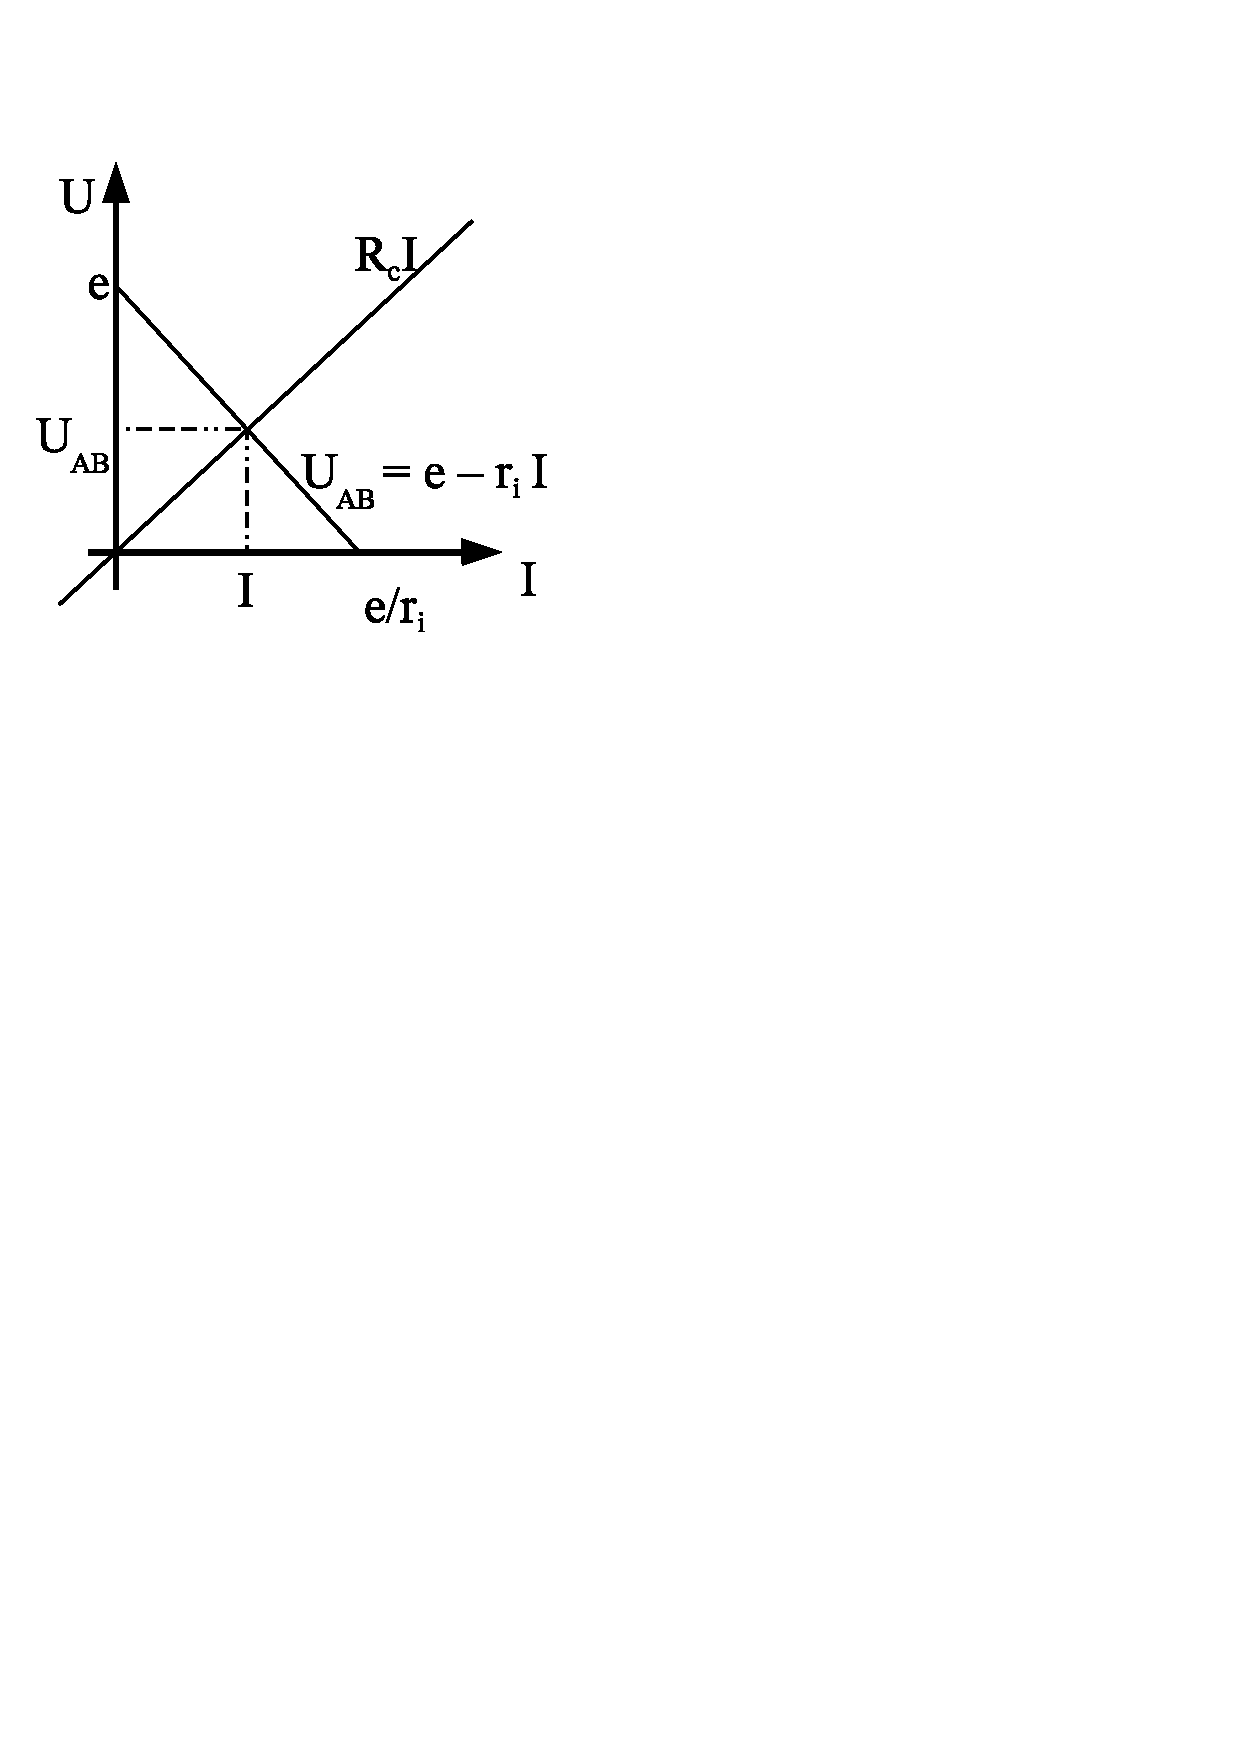
\includegraphics[clip=true,viewport=0cm 19cm 9.5cm 28cm,scale=0.7]{./figures/point_de_fonctionnement.pdf}
\caption{Point de fonctionnement.}\label{fig_pdf}
\end{center}
\end{figure}


\subsubsection{G�n�rateur de tension}

Si la r�sistance de charge $R_{c}$ est tr�s grande devant $r_{i}$, la tension aux bornes du g�n�rateur est sensiblement ind�pendante de $R_{c}$. On obtient alors un g�n�rateur � tension constante dont la courbe caract�ristique est donn�e � la figure \ref{fig_gen_ten}.

\begin{figure}[h]
\begin{center}
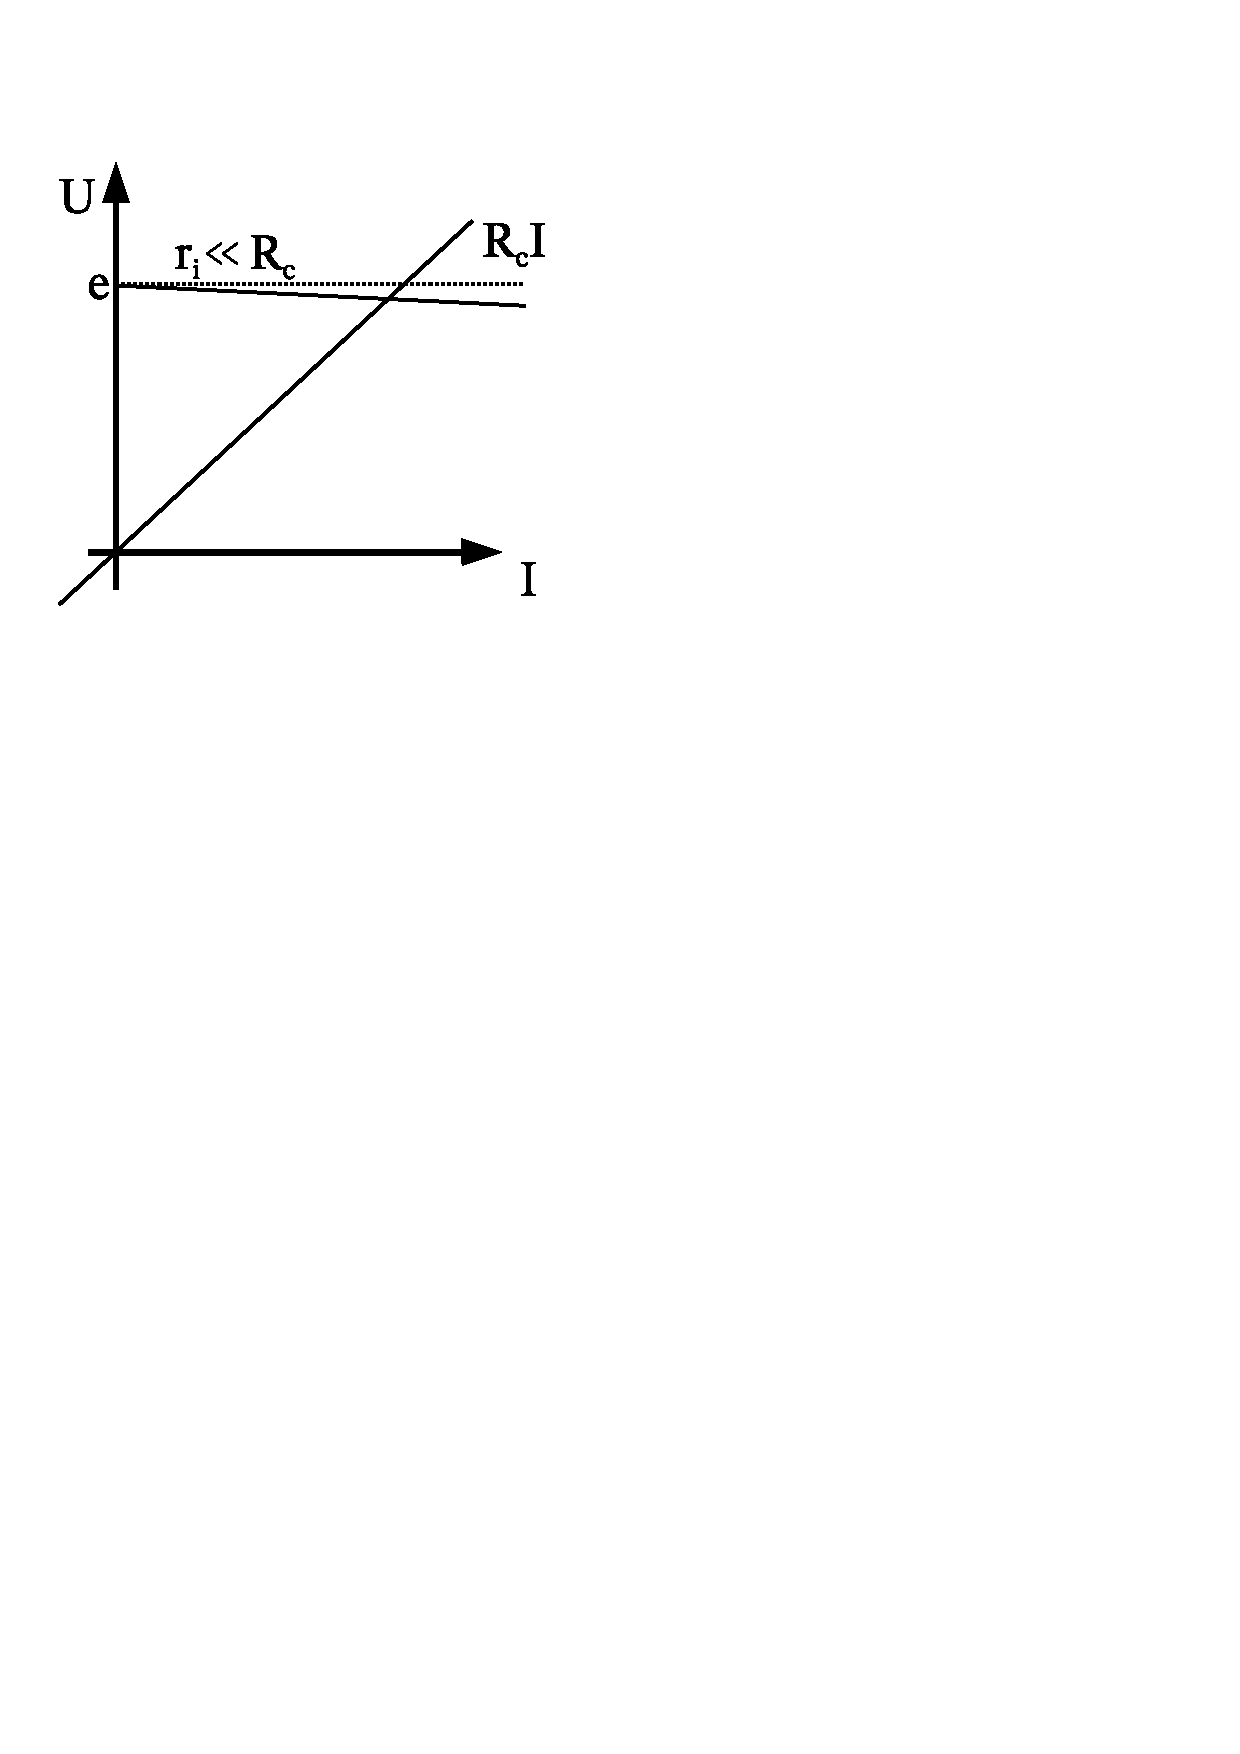
\includegraphics[clip=true,viewport=0cm 19cm 9.5cm 28cm,scale=0.6]{./figures/relation_tension_courant1.pdf}
\caption{Relation tension - courant $U=f(I)$ pour un g�n�rateur de tension.}\label{fig_gen_ten}
\end{center}
\end{figure}

On en d�duit~: $U = e - r_{i}I\approx e$.
Plus la r�sistance $r_{i}$ est petite, plus le g�n�rateur est capable de fournir un courant fort et plus la tension sera proche de $e$.


\subsubsection{G�n�rateur de courant}

Si la r�sistance de charge $R_{c}$ est tr�s petite devant $r_{i}$, alors $i=\fractext{e}{r_{i}+R_{c}}\approx \fractext{e}{r_{i}}$ est ind�pendant de la charge. On obtient alors un g�n�rateur de courant constant dont la courbe caract�ristique est donn�e � la figure \ref{fig_gen_cour}.

\begin{figure}[h]
\begin{center}
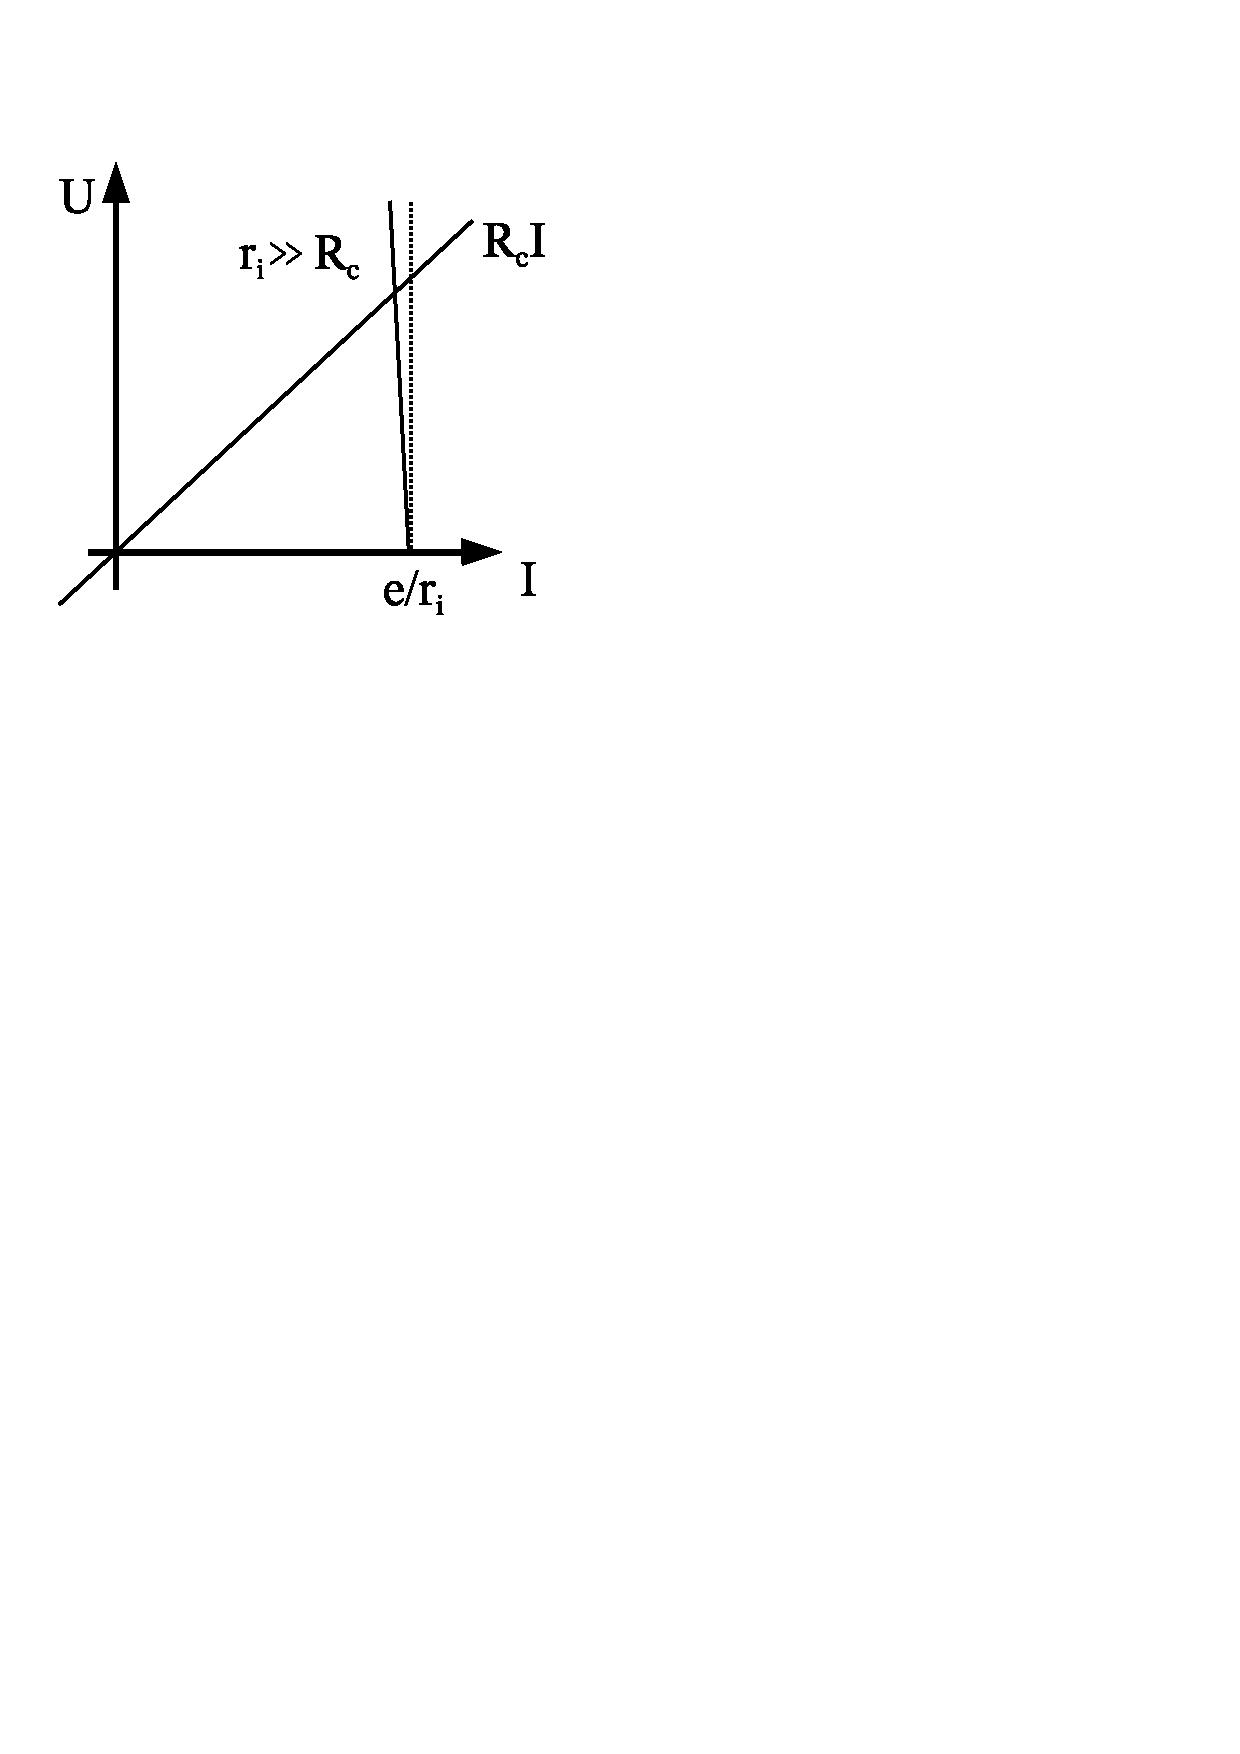
\includegraphics[clip=true,viewport=0cm 19cm 9.5cm 28cm,scale=0.6]{./figures/relation_tension_courant2.pdf}
\caption{Relation tension / courant~: $U=f(I)$ pour un g�n�rateur de courant.}\label{fig_gen_cour}
\end{center}
\end{figure}


\begin{figure}[h]
\begin{center}
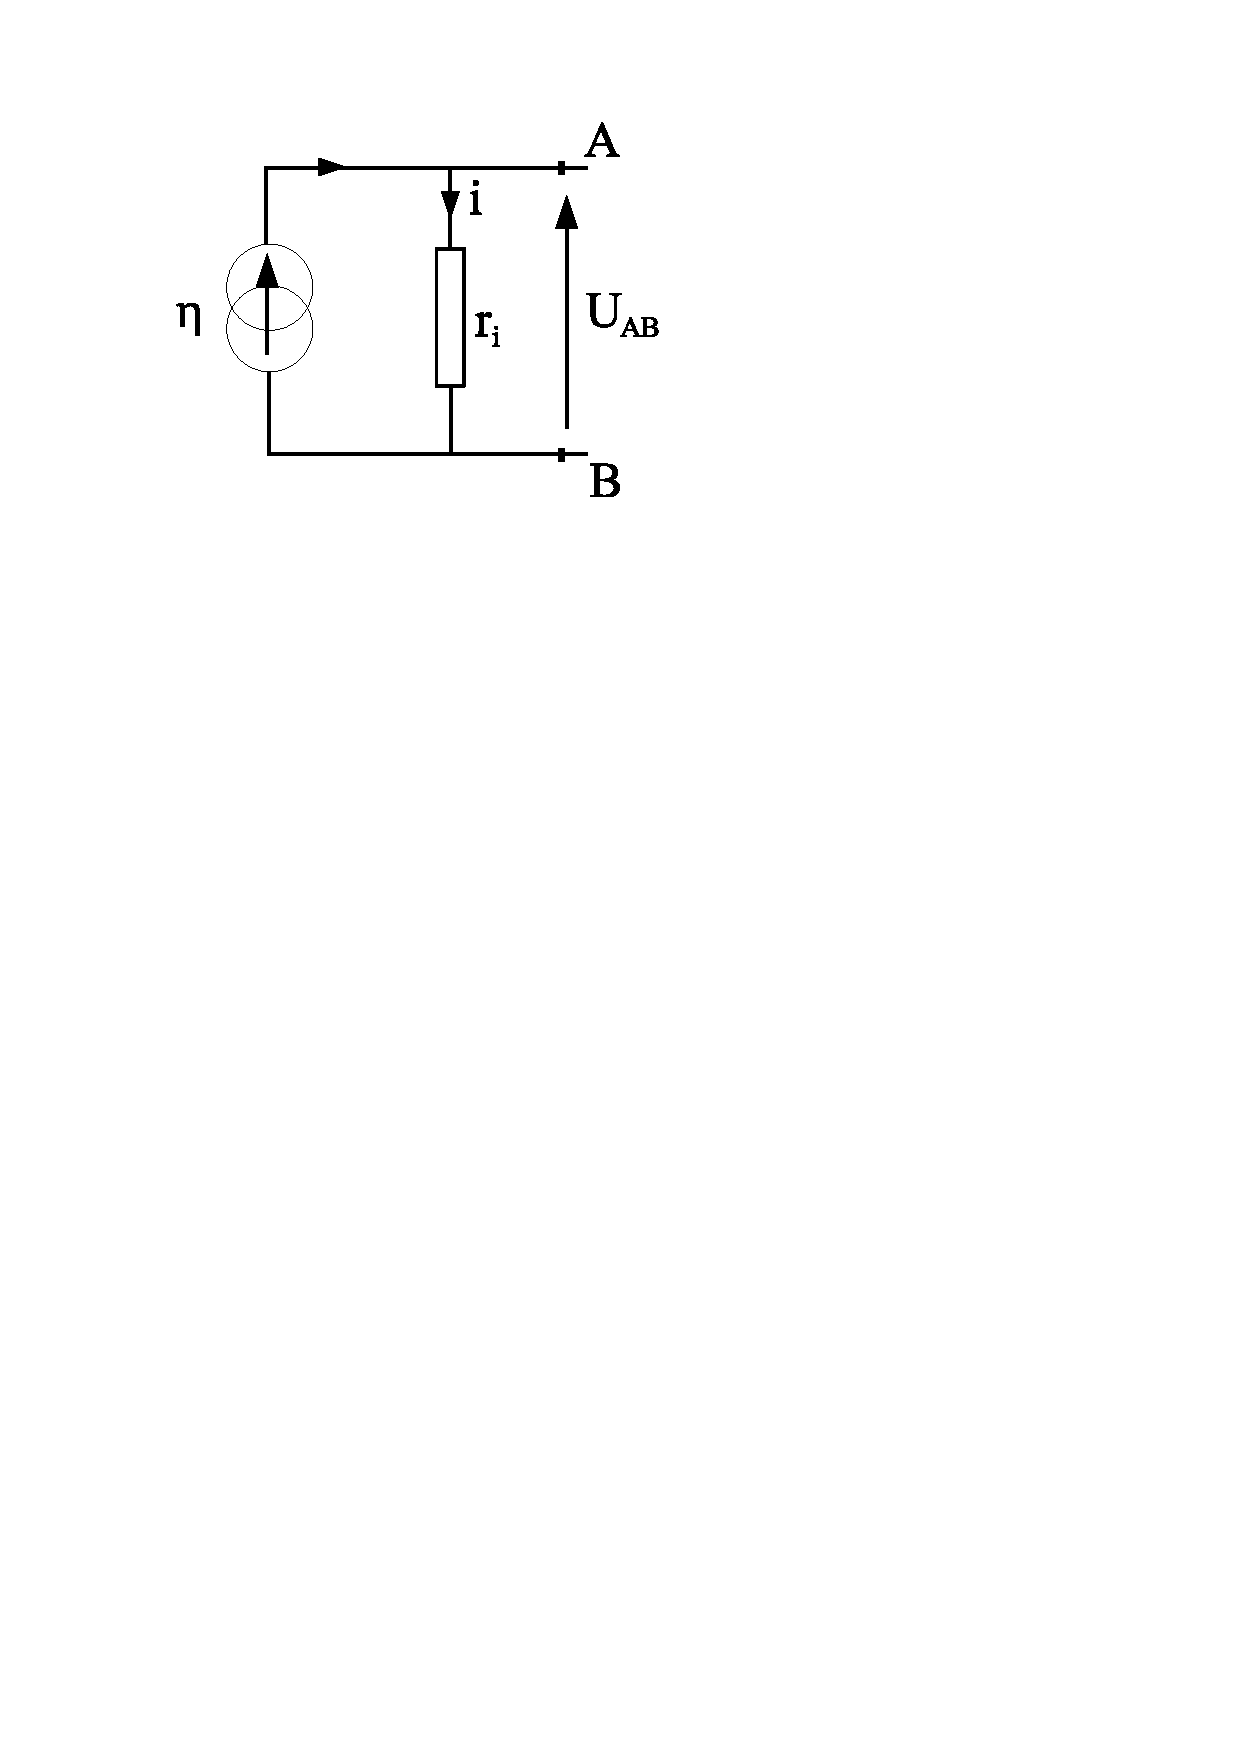
\includegraphics[clip=true,viewport=3cm 20cm 12cm 28cm,scale=0.6]{./figures/generateur_de_courant.pdf}
\caption{G�n�rateur de courant.}\label{sch_gen_cour}
\end{center}
\end{figure}

$\eta $ est le courant fournit par le g�n�rateur quand il y a court-circuit. En g�n�ral, l'imp�dance interne est une r�sistance $r_{i}$ d'o�~: $I = \eta  - \fractext{U}{r_{i}}$, avec $\eta = \fractext{e}{r_{i}}$.

Ici, plus la r�sistance est grande, plus le g�n�rateur est capable de d�livrer un courant proche de $\eta $. La symbolique utilis�e pour sch�matiser ce type de g�n�rateur est pr�sent�e � la figure \ref{sch_gen_cour}.


\subsubsection{Repr�sentation Duale}
L'�quivalence entre les deux repr�sentations est appel�e \textbf{dualit�}. En effet, on peut �crire � la fois :

$$U = e - r_{i} I$$

et

$$I = \frac{e}{r_{i}}-\frac{U}{r_{i}}=\eta  - g_{i}U$$

en posant $\eta =\fractext{e}{r_{i}}$ et $g_{i}=\fractext{1}{r_{i}}$. $e$ et $\eta $ sont orient�s dans le m�me sens. Le principe de dualit� sch�matis� est donn� � la figure \ref{sch_dual}.

\begin{figure}[h]
\begin{center}
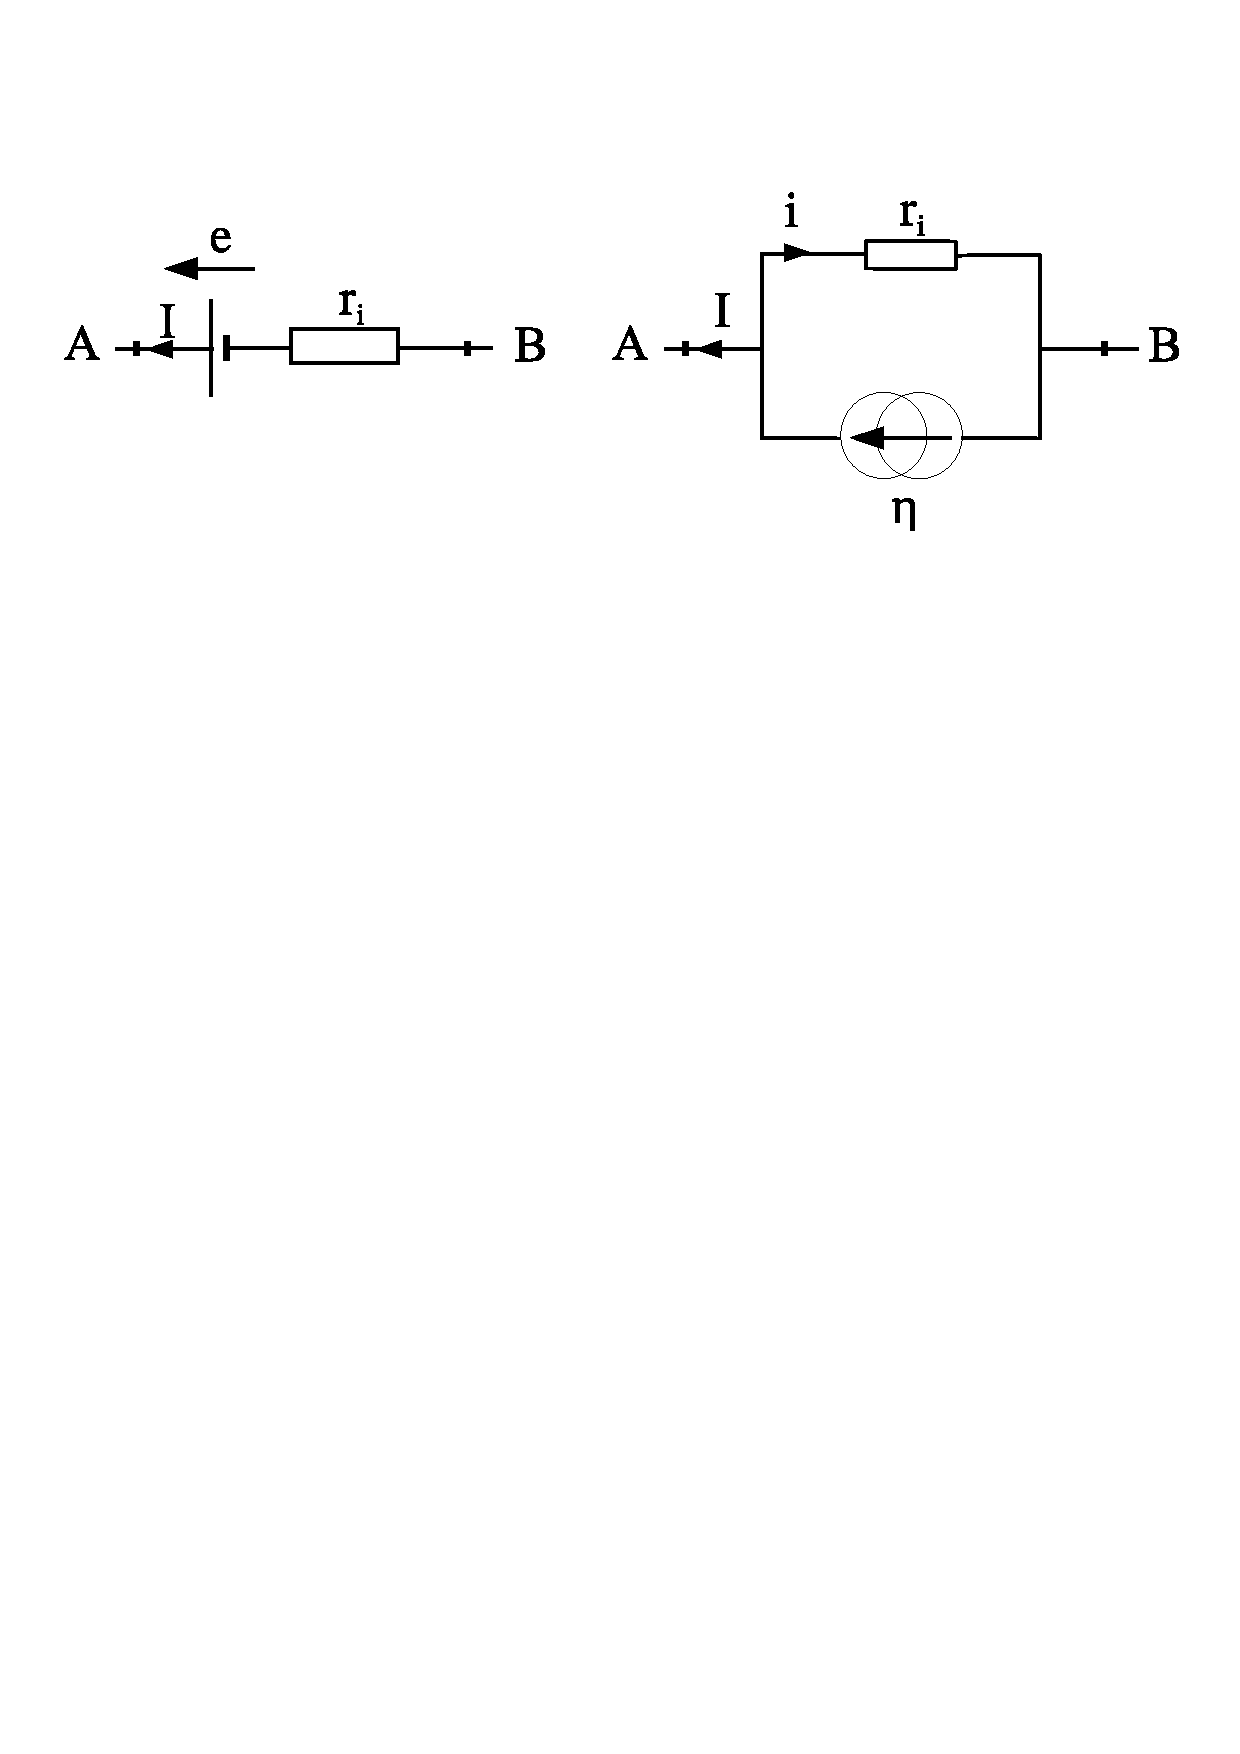
\includegraphics[clip=true,viewport=0cm 20cm 21cm 27cm,scale=0.5]{./figures/representation_duale.pdf}
\caption{Dualit� g�n�rateurs de tension / courant.}\label{sch_dual}
\end{center}
\end{figure}

\begin{itemize}
 \item  G�n�rateur de tension~:

$$U_{AB}=R_{c} I$$
$$I = \frac{E}{R_{i}+R_{c}}$$
$$U_{AB}=\frac{R_{c}}{R_{i}+R_{c}} E$$

 \item G�n�rateur de courant~:

$$\eta =I+i$$
$$I=\eta - \frac{U_{AB}}{r_{i}} I$$
$$I(1+\frac{R_{c}}{r_{i}})=\eta$$
$$I=\frac{r_{i}}{r_{i}+R_{c}} \eta$$

$$I = \frac{1}{r_{i}+R_{c}} e$$
$$U_{AB}=R_{c} I$$
$$U_{AB}=\frac{R_{c}}{R_{i}+R_{c}} E$$
\end{itemize}

On peut r�sumer l'effet de la dualit� ainsi : quand un g�n�rateur de f�m $E$ et de r�sistance interne $R_{i}$ d�bite dans une r�sistance de charge $R_{c}$~:

\begin{itemize}
\item si $r_{i} \ll R_{c}$, alors c'est une source de tension de f�m $E$ ;
\item si $r_{i} \gg R_{c}$, alors c'est une source de courant $I = \fractext{e}{r_{i}}$.
\end{itemize}


\subsubsection{Associations de dip�les~: dip�les �quivalents}

\begin{itemize}
\item Association en s�rie~:

Tension~: $u = \sum_{k} u_{k}$ (somme alg�brique sur une branche)
Source de tension~: $e = \sum_{k} e_{k}$ (somme alg�brique)
R�sistance~: $R = \sum_{k} R_{k}$

De mani�re g�n�rale~: $u = \sum_{k} u_{k} = \sum_{k} e_{k} + (\sum_{k} R_{k}) I$.

\begin{note}L'association en s�rie de sources de courant id�ale n'a aucun sens.
\end{note}

\item Association en parall�le~:

Courant~: $I = \sum_{k} I_{k}$ (somme alg�brique � un n\oe ud)
Conducteur ohmique~: $G = \sum_{k} G_{k}$ (conductance �quivalente)

De mani�re g�n�rale~: $i = \sum_{k} i_{k} = \sum_{k} \eta_{k} + (\sum_{k} G_{k}) U$.

\begin{note} L'association en parall�le de sources de tension id�ales n'a aucun sens.
\end{note}

\end{itemize}


\subsubsection{Adaptation d'imp�dance~: charge adapt�e}

Soit un g�n�rateur de tension dans une r�sistance $R_{c}$.

\begin{figure}[h]
\begin{center}
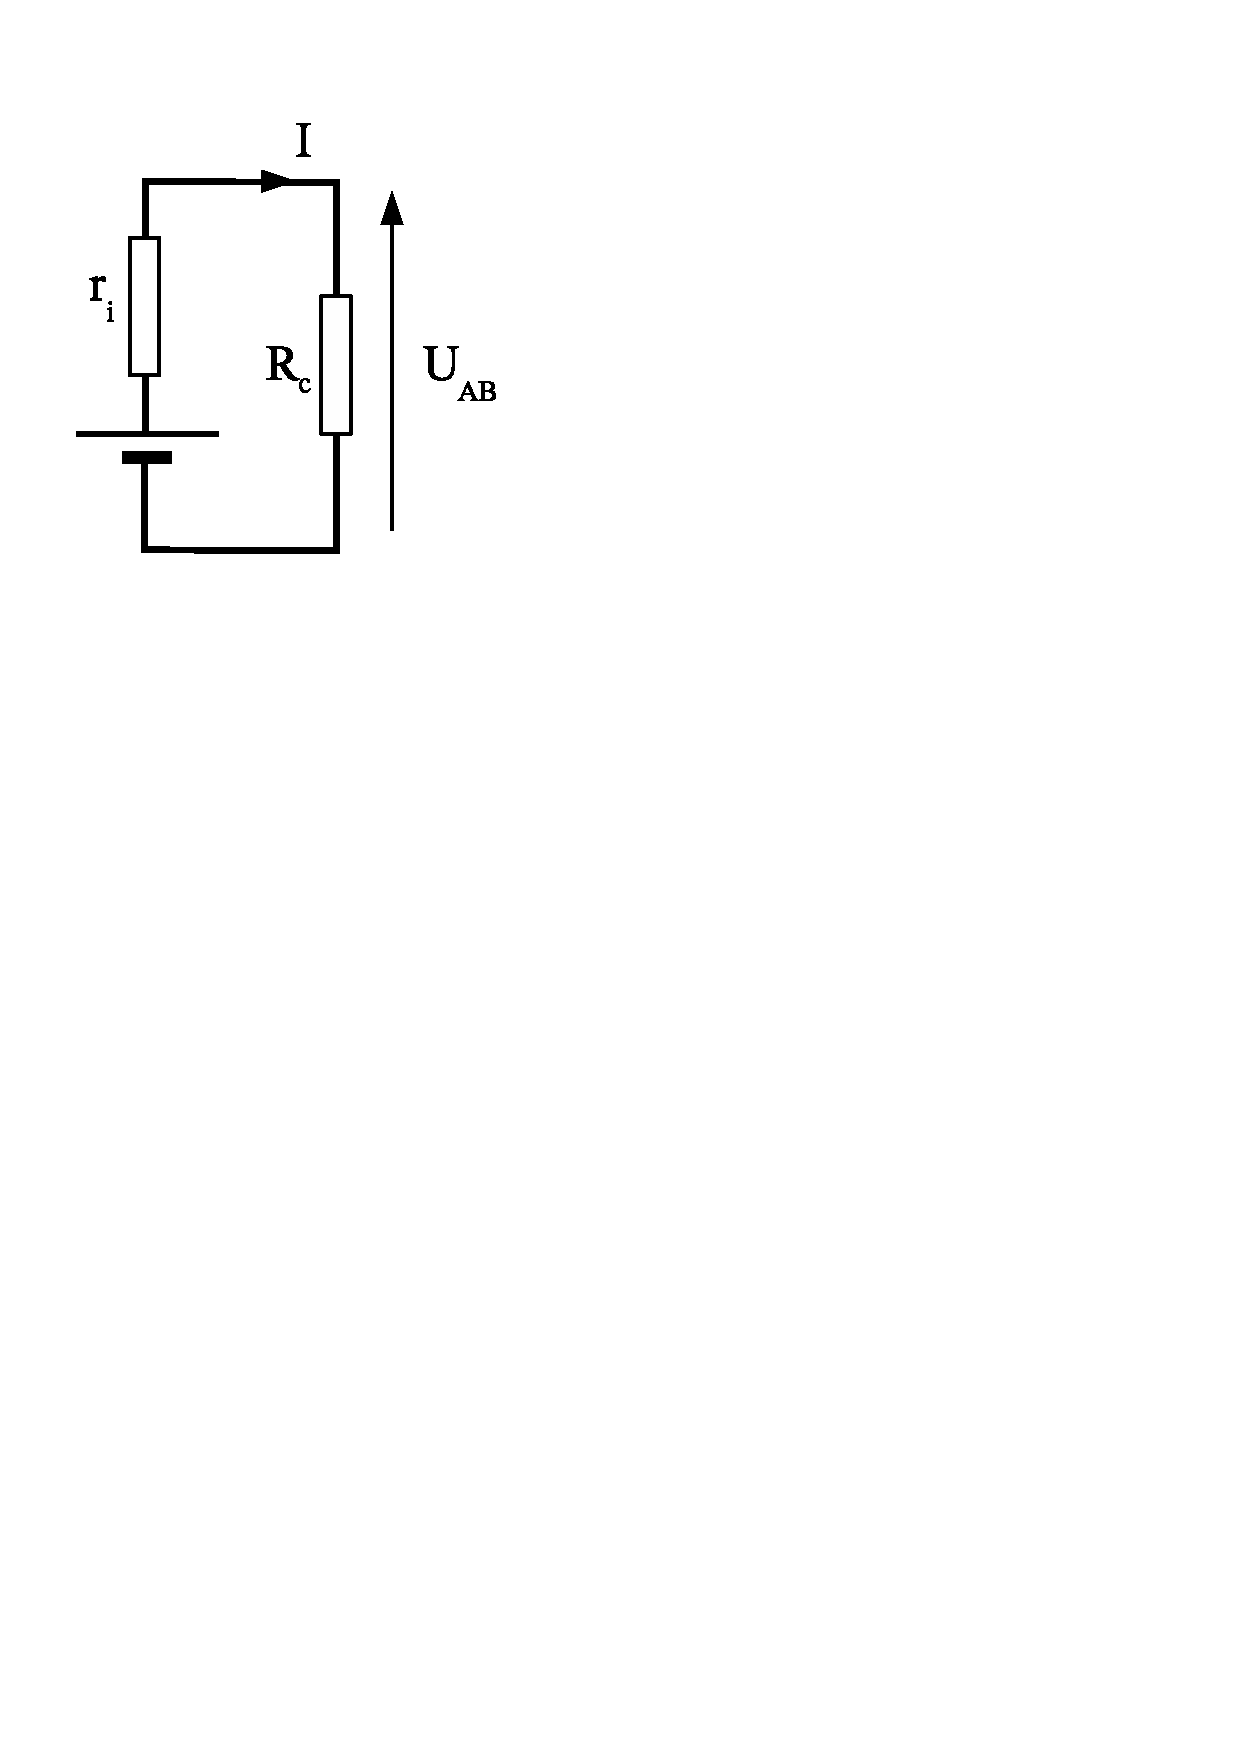
\includegraphics[clip=true,viewport=0cm 20cm 10cm 27cm,scale=0.38]{./figures/circuit_charge.pdf}
\caption{G�n�rateur de tension charg�.}
\end{center}
\end{figure}

$$ \left\{
\begin{array}{ll}
U_{AB}=e-r_{i}I \\
U_{AB}=R_{c} I
\end{array} \right.
$$

$$U_{AB}=e-\frac{r_{i}}{R_{c}} U_{AB}$$

$$e = \frac{R_{c}+r_{i}}{R_{c}} U_{AB}$$

$$U_{AB} = \frac{R_{c}}{R_{c}+r_{i}} e \qquad \textrm{et} \qquad I=\fractext{e}{R_{c}+r_{i}}$$


\begin{description}

\item[Puissance dissip�e dans $r_{i}$]
$$P_{c}=UI=r_{i} I^{2}$$

Nous avons~:
$$P_{c}=\frac{r_{i}}{(R_{c}+r_{i})^2} e^{2}$$

\item[Puissance dissip�e dans $R_ {c}$]
$$P_{c}=U_{AB}I=R_{c} I^{2}$$
avec $I=\fractext{e}{R_{c}+r_{i}}$.

Nous avons~:
$$P_{c}=\frac{R_{c}}{(R_{c}+r_{i})^2} e^{2}$$


Quelle doit �tre la r�sistance de charge pour que la puissance soit maximale ?

\begin{figure}[h]
\begin{center}
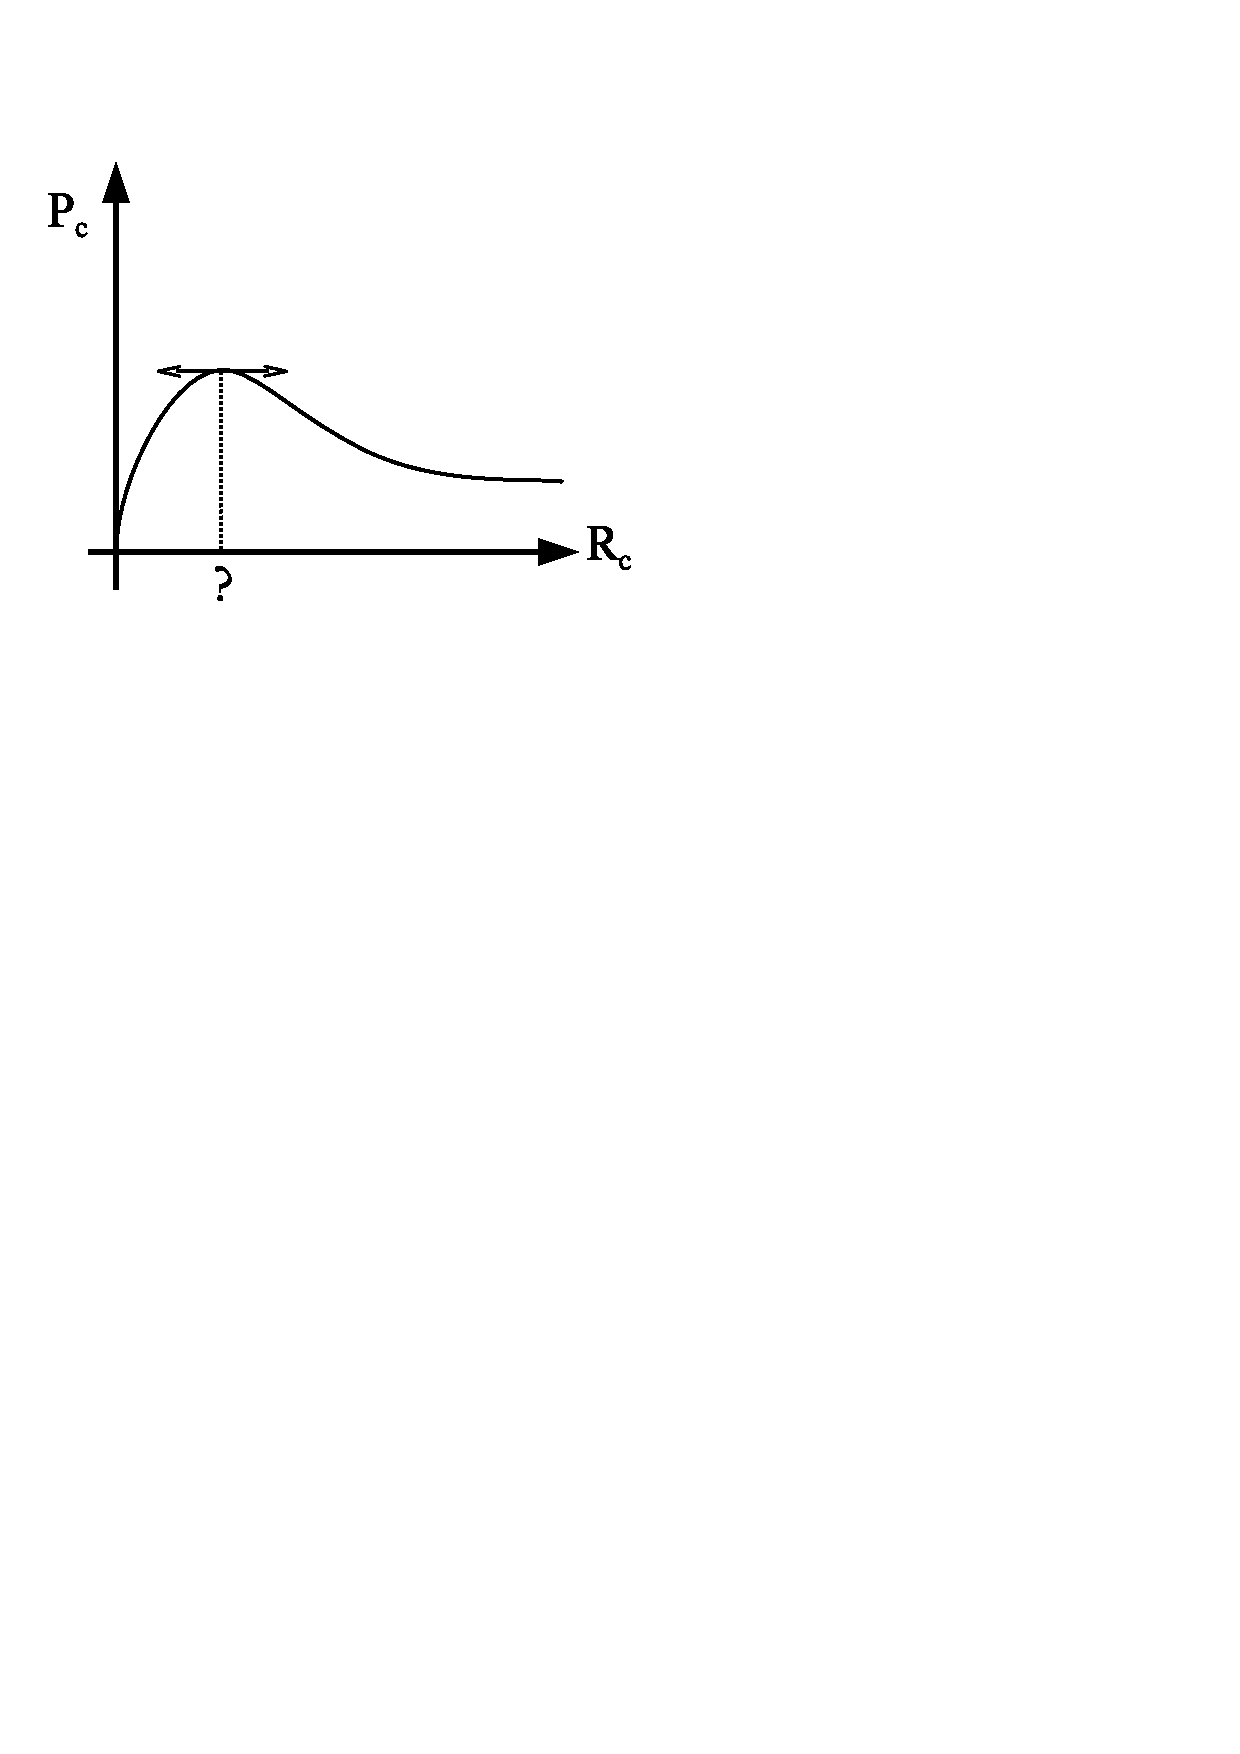
\includegraphics[clip=true,viewport=0cm 18cm 12cm 27cm,scale=0.5]{./figures/puissance_fournie.pdf}
\caption{Puissance fournie.}
\end{center}
\end{figure}

$Pc$ est maximum lorsque $\fractext{\partial P_{c}}{\partial R_{c}}=0$, soit~:

\begin{equation*}
\begin{split}
\frac{\partial P_{c}}{\partial R_{c}} & = \frac{R_{c}+R_{i}-2R_{c}}{(R_{c}+r_{i})^{3}} e^{2} \\
& = \frac{R_{c}+r_{i}-2R_{c}}{(R_{c}+r_{i})^{3}} e^{2}
\end{split}
\end{equation*}

donc lorsque $R_{i}=R_{c}$.
\bigskip

\item[Puissance totale]
$$P_{tot}=eI=P_{c}+P_{i}=\frac{e^{2}}{R_{c}+r_{i}}$$
\end{description}


\section{R�seaux �lectriques}


\subsection{Analyse d'un r�seau en r�gime continu - M�thode de Kirchhoff}

L'analyse d'un r�seau consiste � d�terminer l'intensit� du courant qui circule dans chacune des branches ou des diff�rences de potentiel de chaque branche.

\begin{itemize}
\item Si il y a $N$ n\oe uds, il y a $N-1$ �quations de n\oe uds.
\item Si il y a $B$ branches, il y a $B-(N-1)$ �quations des mailles.
\item On cherche $B$ intensit�s.
\end{itemize}

\begin{enumerate}
\item Fl�cher arbitrairement les courants dans les diff�rentes branches, puis les diff�rences de potentiel. On choisi ensuite un sens arbitraire de description de chacune des mailles.
\item Appliquer la loi des n\oe uds.
Il n'y a pas d'accumulations de charges �lectriques � un n\oe ud, ce qui implique que la somme alg�brique des intensit�s des branches connect�es � un n\oe ud est nulle.

\begin{figure}[h]
\begin{center}
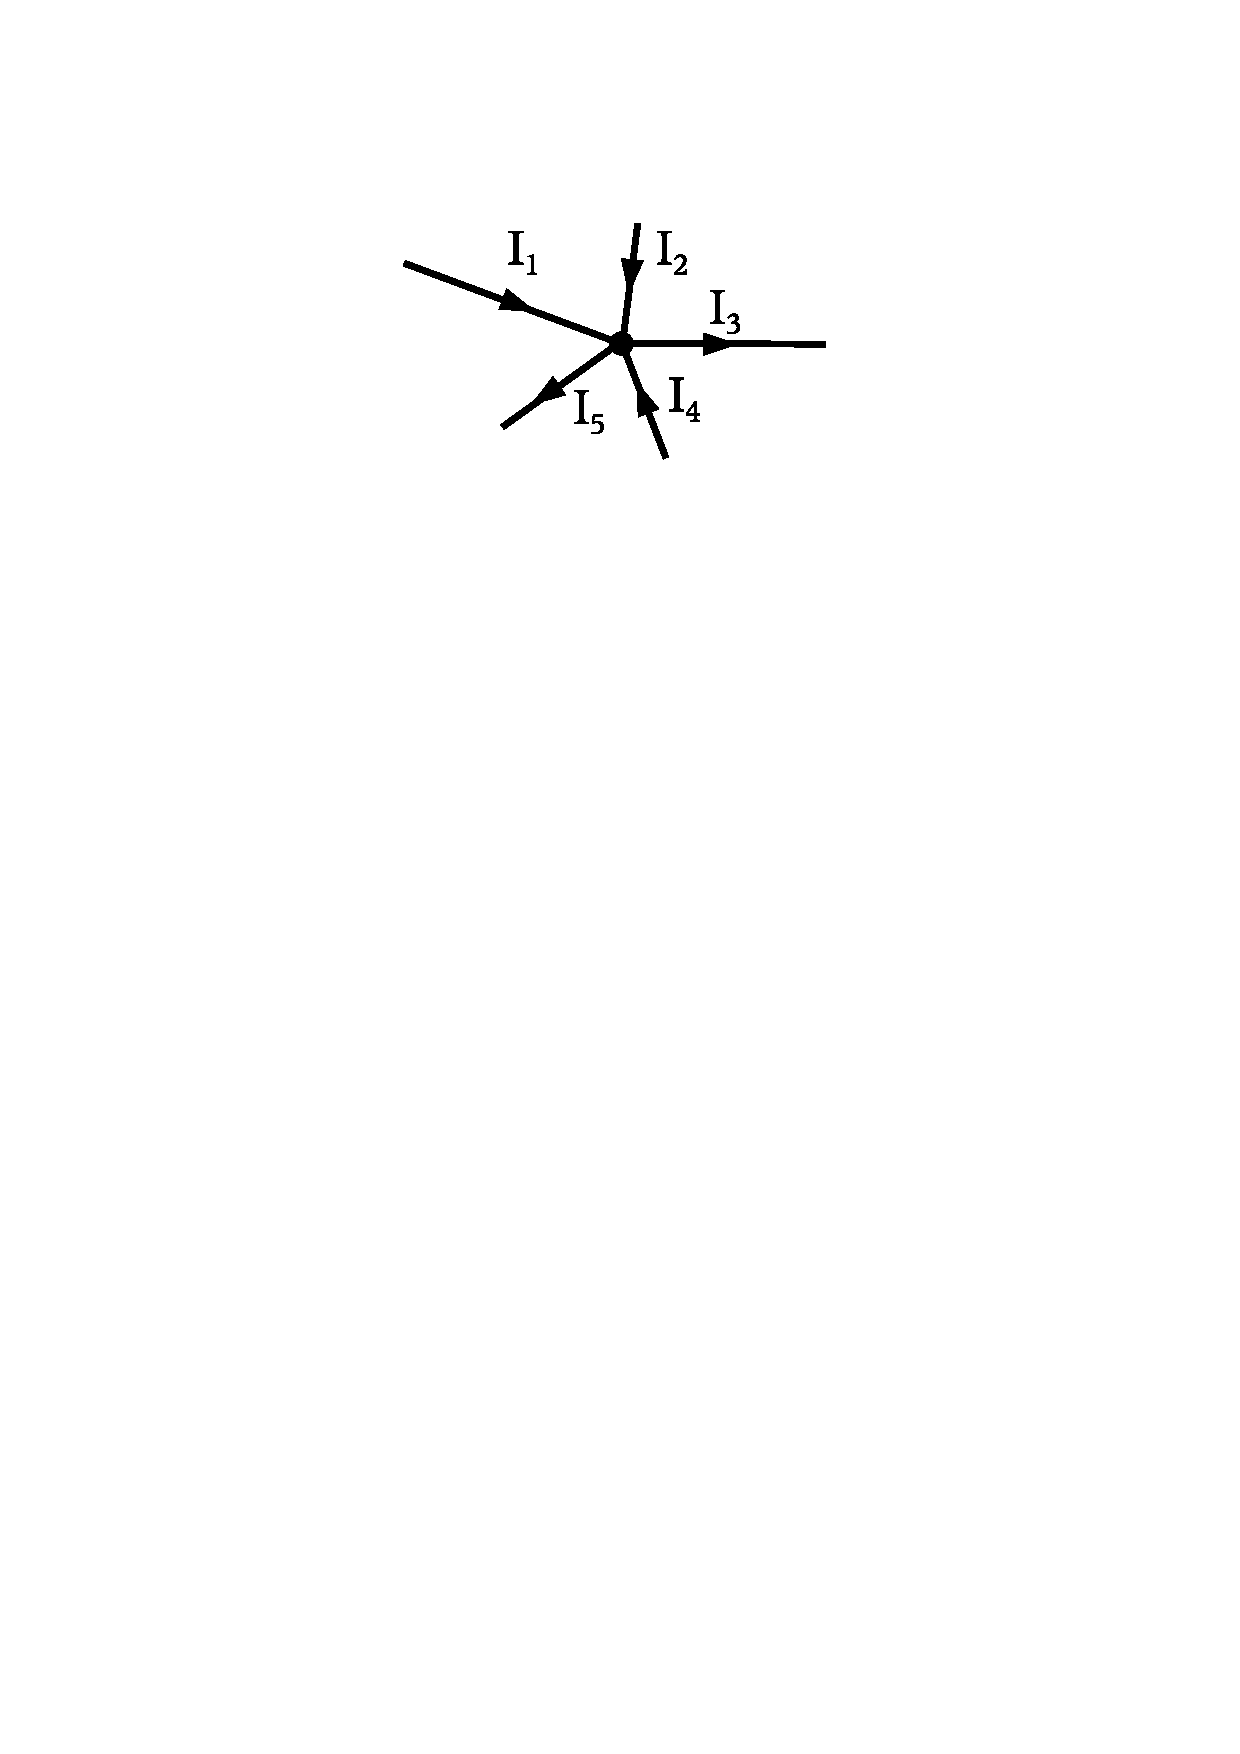
\includegraphics[clip=true,viewport=0cm 22cm 20cm 26cm,scale=0.38]{./figures/loi_des_noeuds.pdf}
\caption{Loi des n\oe uds.}
\end{center}
\end{figure}

$$\sum_{i} I = 0$$

On peut prendre comme convention $+$ si le courant va vers le n\oe ud et $-$ si il en sort.

\item Appliquer la loi des mailles.
En parcourant compl�tement une maille, la somme des diff�rences de potentiels rencontr�s est nulle : $V_{A} - V_{A}$.


\begin{figure}[h]
\begin{center}
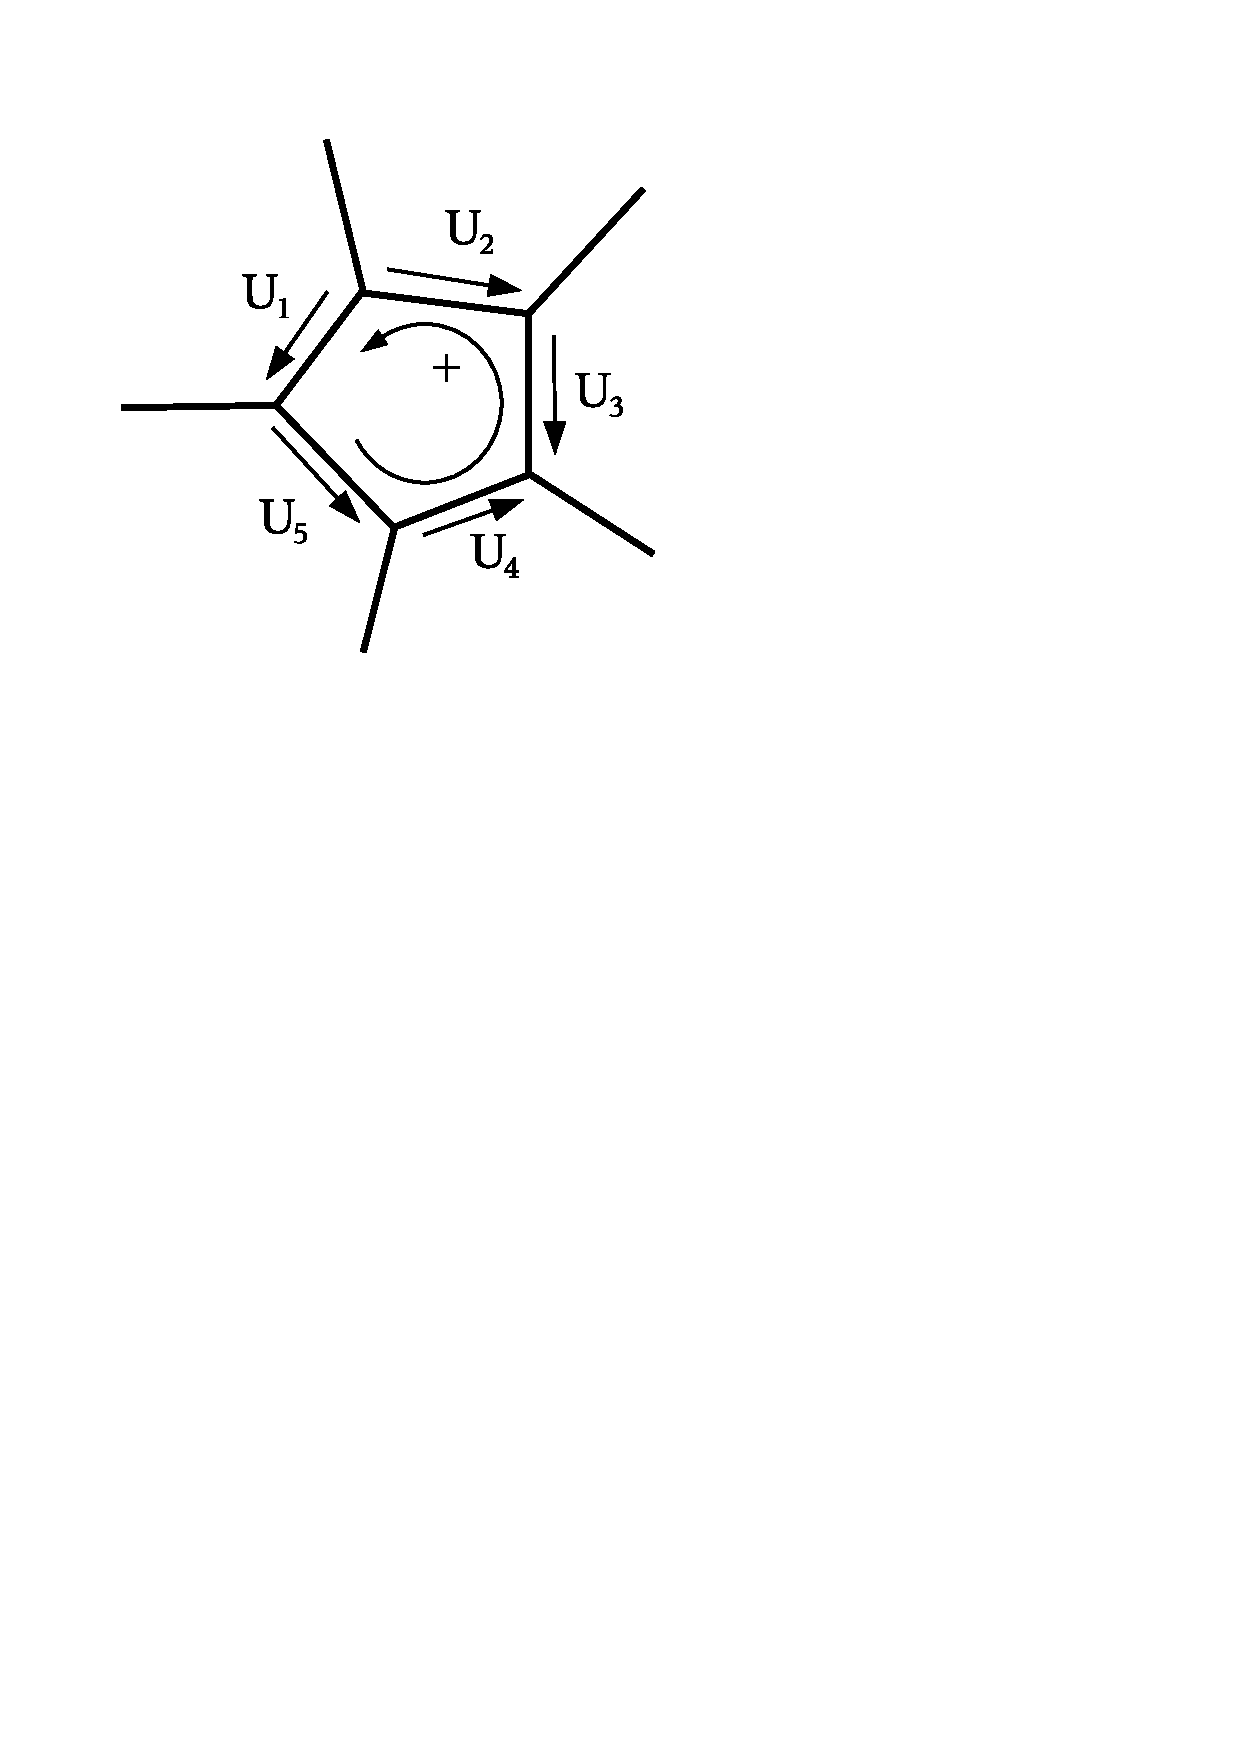
\includegraphics[clip=true,viewport=0cm 18.5cm 18cm 27.5cm,scale=0.55]{./figures/loi_des_mailles.pdf}
\caption{Loi des mailles.}
\end{center}
\end{figure}

$$U_{1}-U_{2}-U_{3}+U_{4}+U_{5}=0.$$


\item R�solution.
Les $B$ �quations obtenues � $B$ inconnues sont r�solues par m�thodes classiques (substitution, d�terminant, ...). Nous obtenons alors des valeurs alg�briques des courants~:
si $I_{i} >0$~: le sens choisi �quivaut au sens r�el ;
si $I_{i} >0$~: le sens choisi est inverse au sens r�el.

\end{enumerate}

\subsection{M�thode de superposition}
Le courant produit dans une branche quelconque d'un r�seau, par un ensemble de sources, est la somme alg�brique des courants produits dans chaque branche par chacune des sources consid�r�es isol�ment, les autres sources �tant rendues passives.
Rendre passives les sources signifit annuler les f�m (court-circuit�es) et les courants �lectromoteurs (circuits ouverts).

Exemple~:

\begin{figure}[h]
\begin{center}
\includegraphics[clip=true,viewport=0cm 23cm 20cm 27cm,scale=0.9]{./figures/methode_superposition.pdf}
\caption{M�thodes de superposition.}
\end{center}
\end{figure}

\subsection{Th�or�me de Millmann}

Ce th�or�me s'applique dans le cas de branche en parall�le.

\begin{figure}[h]
\begin{center}
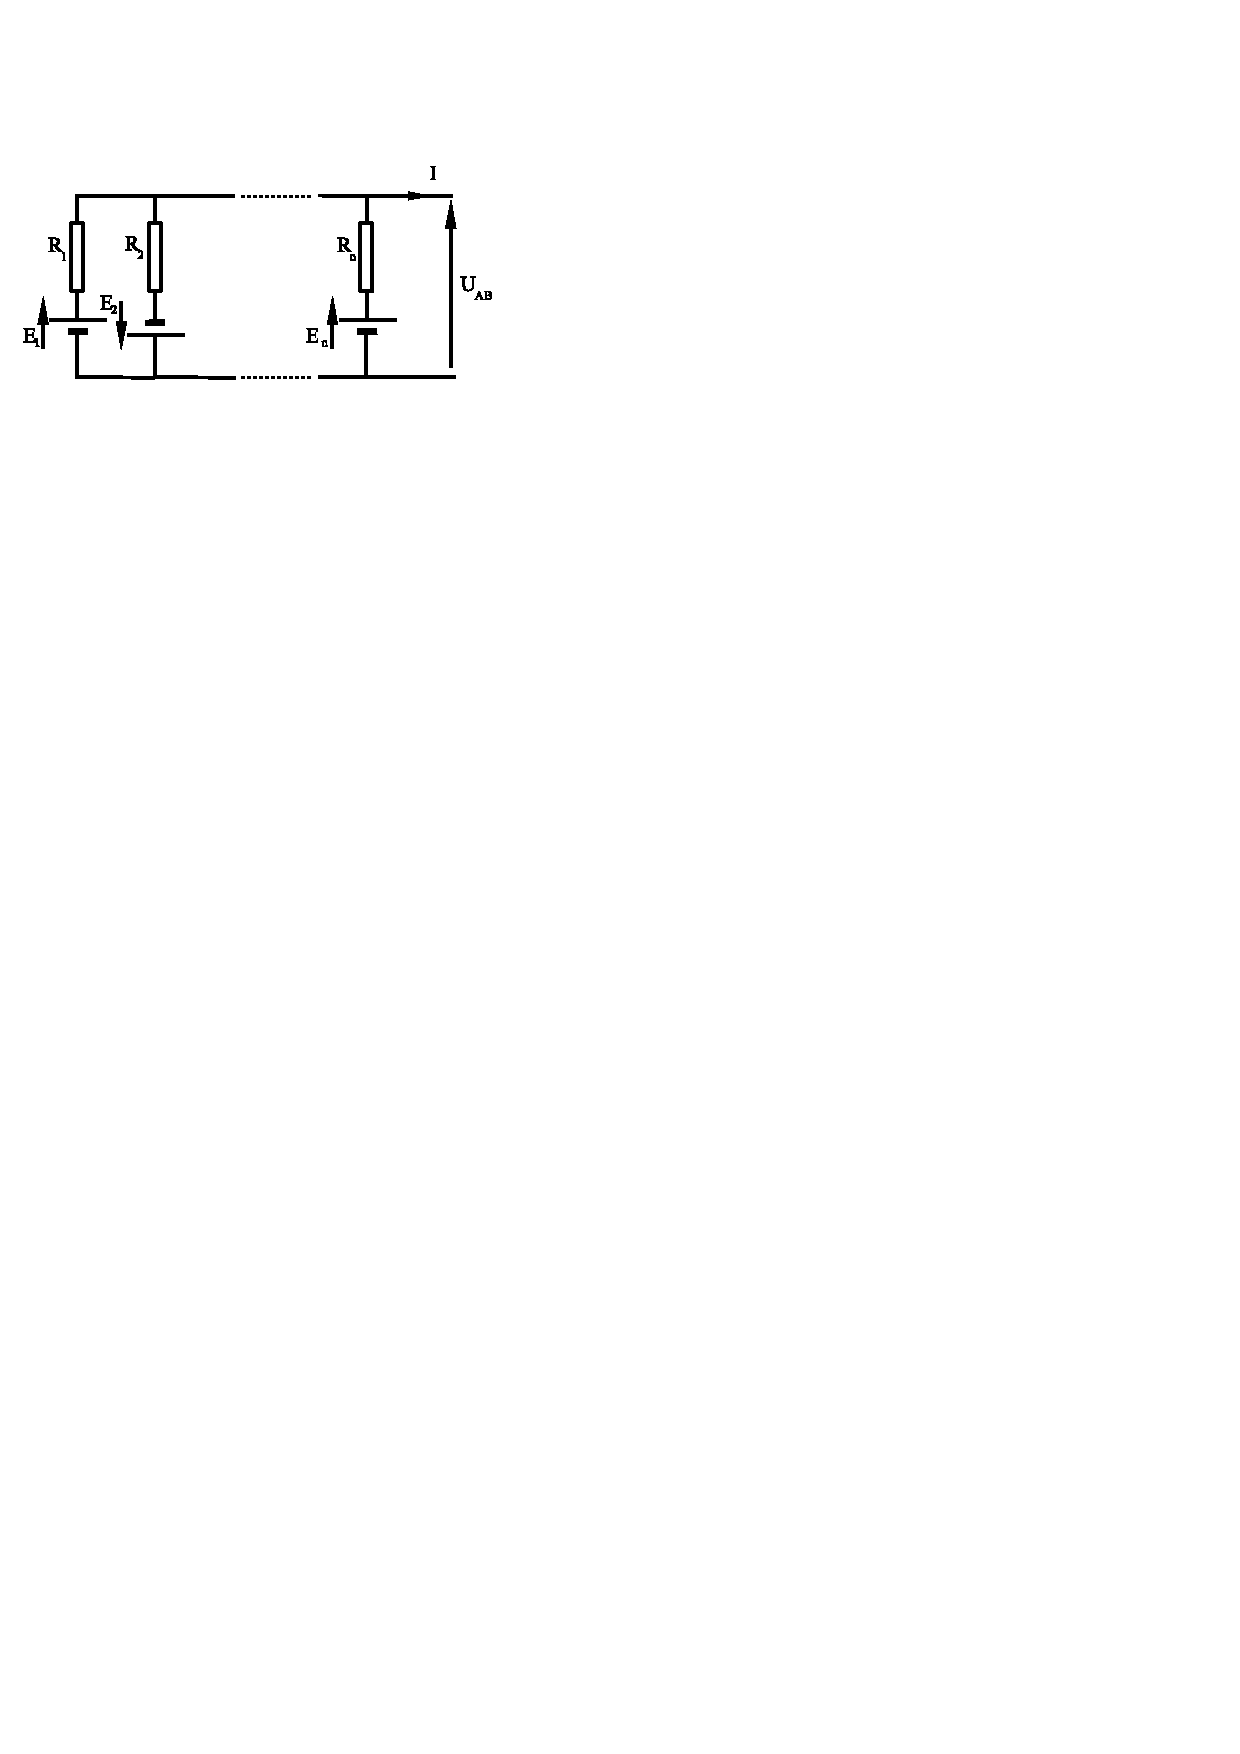
\includegraphics[clip=true,viewport=0cm 23cm 9cm 27cm,scale=1]{./figures/methode_millmann.pdf}
\caption{Th�or�me de Millmann.}
\end{center}
\end{figure}

$$U_{AB} = \fractext{\sum_{i} \pm \fractext{e_{i}}{r_{i}}} {\sum_{i} \fractext{1}{r_{i}}}.$$

La d�monstration par dualit� est �vidente~:

\begin{figure}[h]
\begin{center}
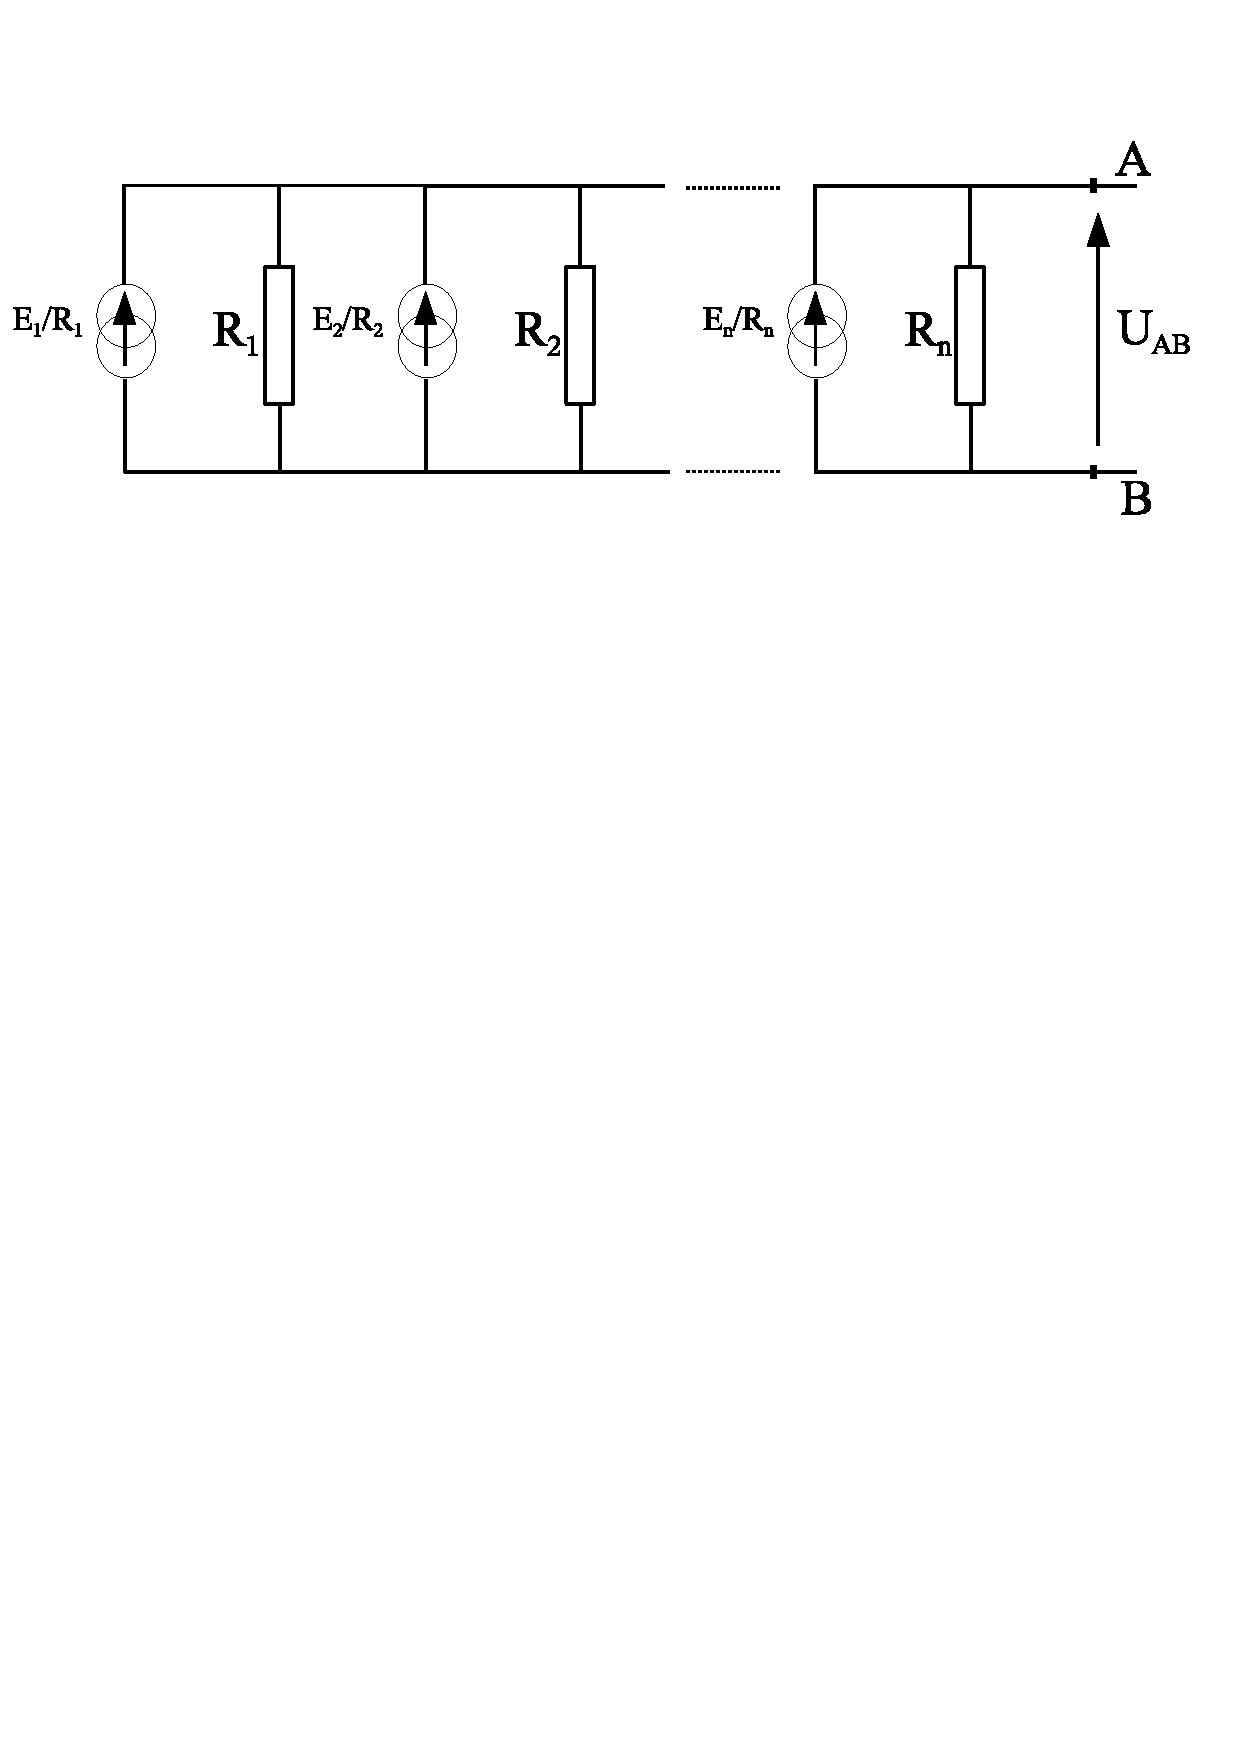
\includegraphics[clip=true,viewport=0cm 21cm 21cm 27.5cm,scale=0.7]{./figures/methode_millmann_dual.pdf}
\caption{Circuit dual �quivalent.}
\end{center}
\end{figure}

$$\frac{1}{R}=\sum_{i} \frac{1}{r_{i}}$$
$$I=\sum_{i}I_{i}=\sum_{i}\frac{e_{i}}{r_{i}}$$
$$U_{AB}=RI$$

\subsection{Th�or�me de Th�venin}

\begin{enon}
Tout r�seau lin�aire compris entre deux bornes $A$ et $B$, aussi compliqu� soit-il, est �quivalent � un g�n�rateur unique de f�m $e$ et de r�sistance interne $r$ telles que :
\begin{enumerate}
\item $e = E$ est la tension mesur�e entre $A$ et $B$ � l'aide d'un voltm�tre ;
\item $r = R_{eq}$, o� $R_{eq}$ est la r�sistance �quivalente du r�seau, obtenue en posant que toutes les forces �lectromotrices (f.�.m.) et les forces contre-�lectromotrices (f.c.�.m.) sont nulles.
\end{enumerate}
\end{enon}

On ne s'int�resse qu'au fonctionnement d'un dip�le �quivalent $(AB)$ d'un r�seau. Si ce dip�le �quivalent est une source de tension, on l'appelle g�n�rateur de Th�venin. Cette m�thode est donc tr�s utile pour d�terminer des g�n�rateurs �quivalents de circuits complexes pour lesquels les lois de Kirchhoff deviennent inadapt�es, \cad lorsque le nombre d'inconnues dans le syst�me d'�quations devient trop grand.


 \begin{figure}[h]
\centering
\subfigure[Sch�ma initial]{\includegraphics[width=5cm]{./figures/sch_thev_1-crop.pdf}}
\subfigure[]{\includegraphics[width=2cm]{./figures/implique.pdf}}
\subfigure[G�n�rateur de Th�venin �quivalent]{\includegraphics[width=5cm]{./figures/sch_thev_5-crop.pdf}}
\caption{Exemple d'un sch�ma pour l'application du th�or�me de Th�venin.}
\label{sch_thev_1}
\end{figure}

\begin{bex}[Cicuit �quivalent]

La figure \ref{sch_thev_1} pr�sente une r�sistance $R$ aliment�e par un circuit comprenant un g�n�rateur $E$ muni de sa r�sistance propre $R1$ et d'une r�sistance suppl�mentaire $R2$ en parall�le. On cherche � conna�tre le g�n�rateur �quivalent aux bornes de $R$ entre $A$ et $B$.

% \begin{figure}[h]
% \begin{center}
% 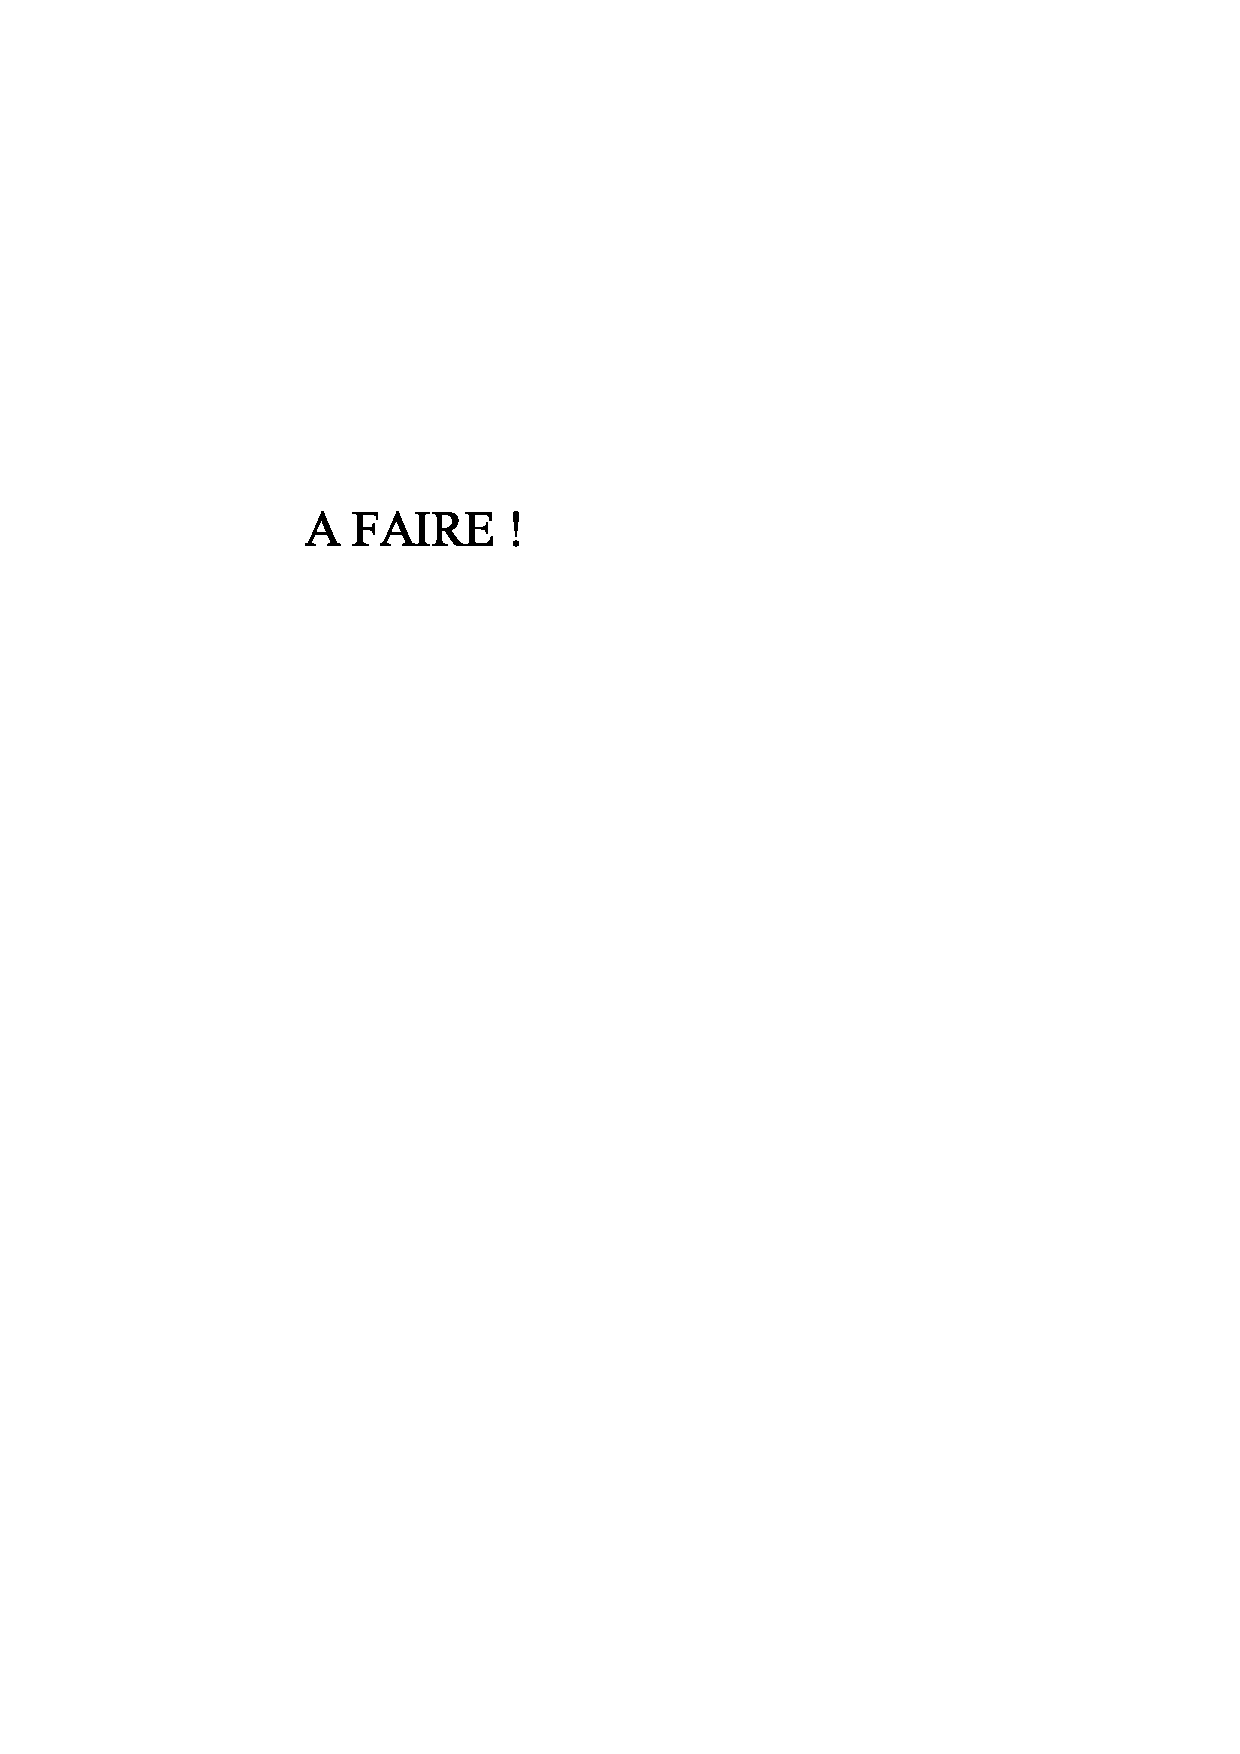
\includegraphics[clip=true,viewport=0cm 18cm 20cm 27cm,scale=0.38]{./figures/a_faire.pdf}
% \caption{Exemple de circuit charg�.}
% \end{center}
% \end{figure}

L'application du th�or�me de Th�venin comporte 4 �tapes.

\begin{enumerate}

\item On d�connecte le dip�le de charge (cf. \ref{sch_thev}(a)):

\begin{figure}[h]
\centering
\subfigure[$1^{\'ere}$ �tape - enl�vement de la charge]{\includegraphics[width=5cm]{./figures/sch_thev_2-crop.pdf}}
\hspace{2cm}
\subfigure[$2^e$ �tape - calcul de la r�sistance �quivalente]{\includegraphics[width=5cm]{./figures/sch_thev_3-crop.pdf}}\\
\subfigure[$3^e$ �tape - calcul de la tension � vide]{\includegraphics[width=5cm]{./figures/sch_thev_2-crop.pdf}}
\hspace{2cm}
\subfigure[$4^e$ �tape - remplacement du dip�le par le g�n�rateur de Th�venin �quivalent]{\includegraphics[width=5cm]{./figures/sch_thev_5-crop.pdf}}
\caption{Etape du calcul d'un g�n�rateur de Th�venin �quivalent.}
\label{sch_thev}
\end{figure}


\item On supprime toutes les sources et on calcule la r�sistance �quivalente $R_{th}$ (cf. \ref{sch_thev}(b)):

\begin{equation}\label{r_th}
R_{th} = \frac{R_{1}R_{2}}{R_{1}+R_{2}}
\end{equation}

\item On r�tablit les sources et on calcule la tension � vide $E{th}=V_A-V_B$ qui donnera la tension du g�n�rateur �quivalent (cf. \ref{sch_thev}(c)):

D'apr�s la loi d'Ohm $I1=I2$ et $I3=0\ A$, d'o�:

\begin{equation}
I1=\frac{E1}{R1+R2}\end{equation}

On en d�duit d'apr�s la loi des mailles :

\begin{equation}\label{e_th}
 E_{th} = V_A - V_B = R2.I2 =  \frac{R2.E1}{R1+R2}
\end{equation}

\item On remplace le dip�le de commande par le g�n�rateur de Th�venin �quivalent (cf. \ref{sch_thev}(d)) o� on utilise les quantit�s donn�es aux �quations \ref{r_th} et \ref{e_th}.

\end{enumerate}

\textbf{Remarque :} ATTENTION ! Ceci est un example et non un cas g�n�ral. Seule la m�thode en 4 �tapes s'applique mais les �quations diff�rent selon les cas. On doit syst�matiquement utiliser les lois de Kirchhoff pour d�terminer les lois de tension et de courant.
\end{bex}


\subsection{Th�or�me de Norton}

C'est la forme duale du th�or�me de Th�venin. Le g�n�rateur de tension est remplac� par un g�n�rateur de courant.

\begin{figure}[h]
\begin{center}
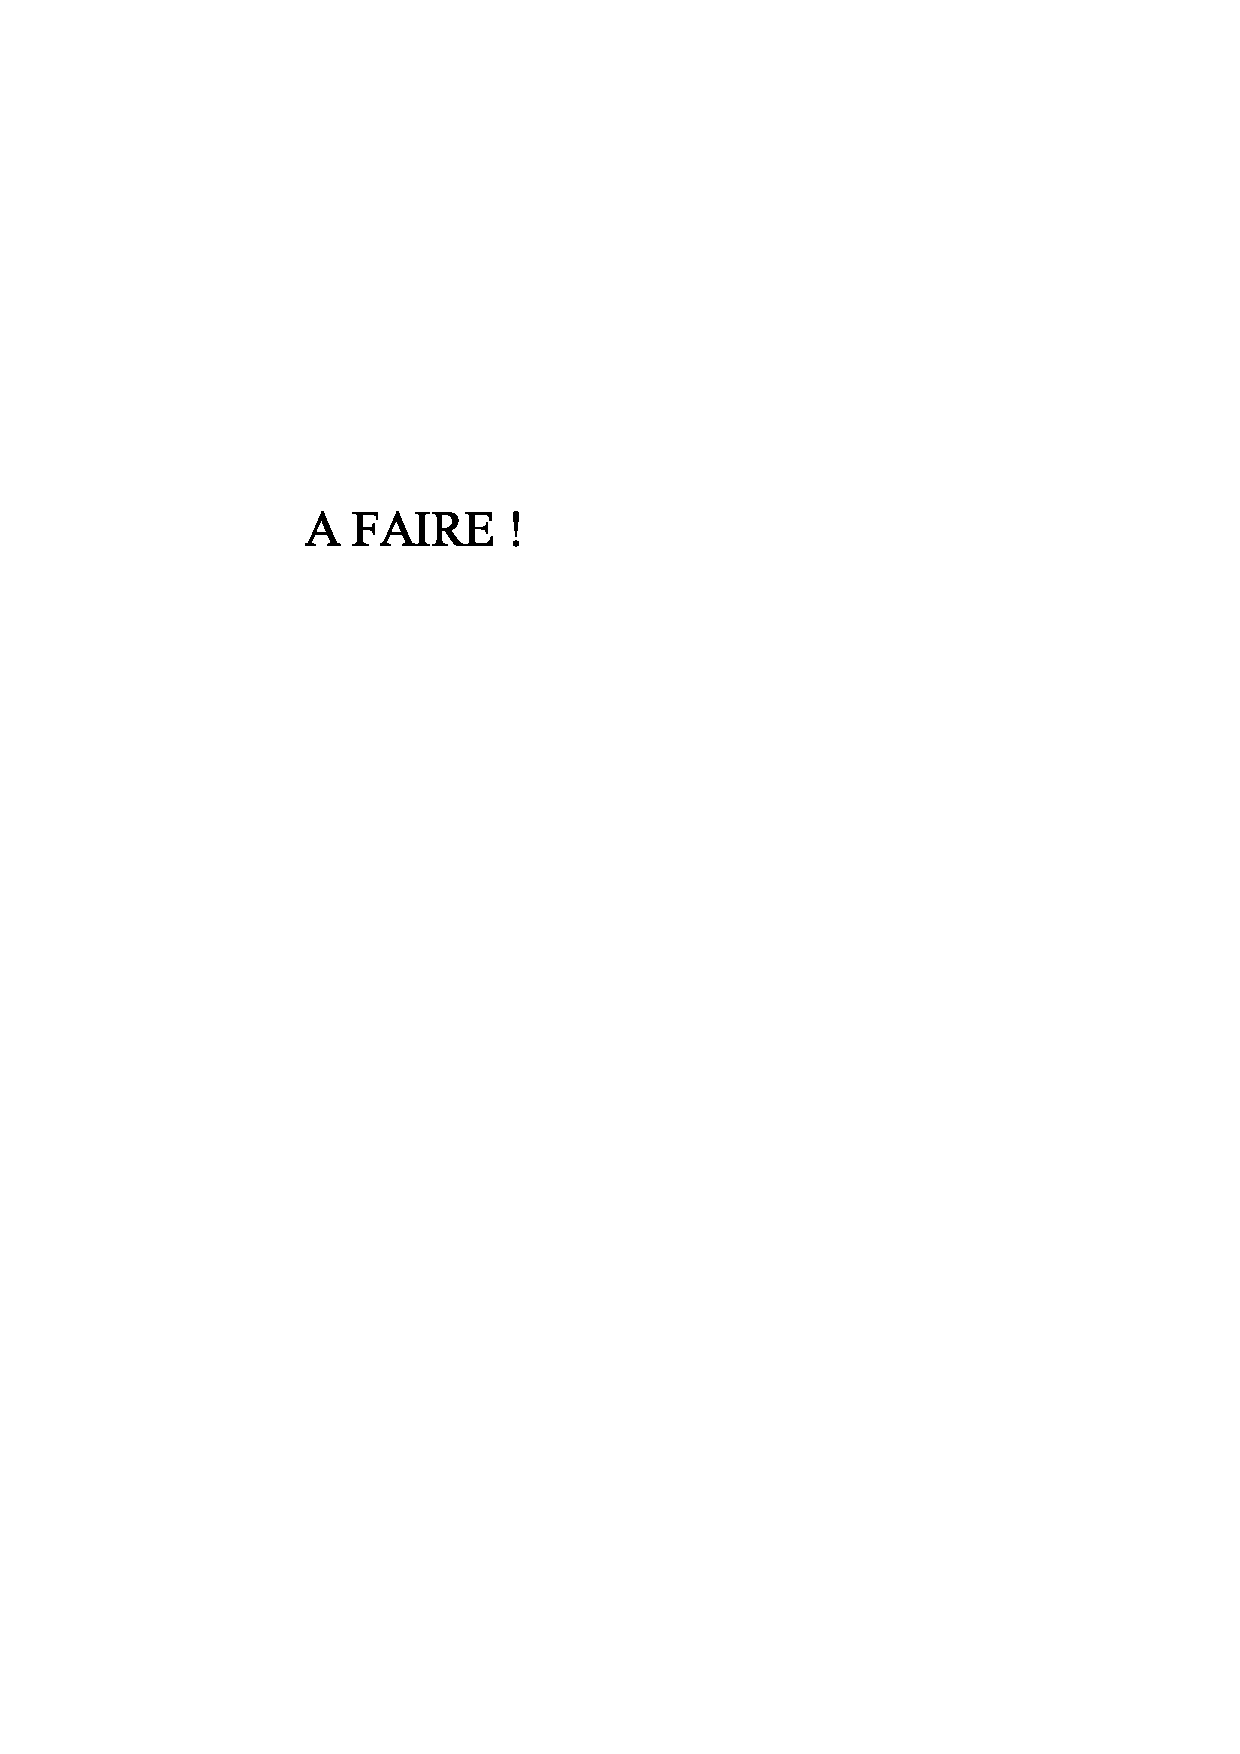
\includegraphics[clip=true,viewport=0cm 18cm 20cm 27cm,scale=0.38]{./figures/a_faire.pdf}
\caption{G�n�rateur de Norton.}
\end{center}
\end{figure}

La r�sistance est d�termin�e de la m�me fa�on. Le courant est le courant de court-circuit pratiqu� aux bornes du dip�le de commande.

\textit{Suite � venir...}

\cleardoublepage

\chapter{Electromagn�tisme}\label{chap_elecmagn}
\input{elec_cpda_cnam-chap_elecromagnetisme}

\chapter{Courants Variables}\label{chap_cour_var}
\input{elec_cpda_cnam-chap_courants_variables}

%%%%%%%%%%%%%%%%%%%%%%%

\newpage
\begin{center}
\bold{\emph{\underline{RESUME DU PROGRAMME D'ELECTRICITE (20 heures)}}}
\end{center}

\bigskip

\bold{\emph{ELECTROSTATIQUE}}

\begin{small}
\begin{enumerate}
\item{Rappels}
	G�n�ralit�s~: charge �lectrique �l�mentaire ; corps charg�s. Loi de Coulomb. Principe de superposition. Champ �lectrique ; exemples.
\item{Etude du champ �lectrique}
	D�finition du flux. Th�or�me de Gauss. Application~: calcul du champ cr�� par une distribution uniforme (rectiligne, plane, sph�rique).
\item{Potentiel}
	Travail des forces �lectriques ; d�finition du potentiel. Relation entre potentiel et champ. Calculs de potentiels simples.
\item{Condensateurs}
	\begin{itemize}
	\item Charge des condensateurs en �quilibre. D�finition et capacit� du condensateur.
	\item Condensateur en pr�sence d'un di�lectrique.
	\item Energie emmagasin�e par un condensateur,
	\item Association de condensateurs
	\end{itemize}
\item Notions sur les �lectrets
\end{enumerate}
\end{small}

\bold{\emph{COURANTS CONTINUS}}

\begin{small}
\begin{enumerate}
\item{Rappels}
	G�n�ralit�s~: densit� de courant, courant, intensit�, diff�rence de potentiel. Loi d'Ohm, r�sistivit� et r�sistance des conducteurs. Association de r�sistances. Loi de Joule.
\item{G�n�rateurs - R�cepteurs}
	\begin{itemize}
	\item G�n�rateur. 	D�finition ; f.e.m., r�sistance interne. G�n�rateur de tension, g�n�rateur de courant. Charge adapt�e. Association. G�n�rateur chimique~: Description et fonctionnement d'une pile. Exemples. Potentiel d'�lectrode.
	\item R�cpeteur. D�finition ; f.e.m., r�sistance interne. Association.
	\end{itemize}
\item{R�seaux}
	D�finitions et conventions de signe internationale. Lois de Kirchoff ; loi des noeuds, loi des mailles. Mise en �quation et r�solution de r�seaux simples. Th�or�me de superposition. Th�or�me de Th�venin et th�or�me de Norton, applications.\\
\end{enumerate}
\end{small}

\bold{\emph{ELECTROMAGNETISME}}

\begin{small}
\begin{enumerate}
\item{Rappels}
	\begin{itemize}
	\item Magn�tostatique
		Origine du champ magn�tique, force de Lorentz.
		Action d'un champ sur un circuit~: loi de Laplace ; exemples.
		Champs cr��s par des courants ; exemples.
		Int�raction entre circuits~: relation entre flux magn�tiques et courants ; coefficients d'inductance. Propri�t�s des aimants permanents.
	\item Induction
		Description du ph�nom�ne. F.e.m. d'induction ; loi de Faraday. Auto-induction ; tension aux bornes d'une bobine. Induction mutuelle ; tension aux bornes de bobines coupl�es.
	\end{itemize}
\item{Etude du champ magn�tique}
Loi de Biot et Savart~: calcul d'un champ cr�� par un fil rectiligne. Th�or�me d'Amp�re. Application au sol�no�de. Notion de conservation du flux magn�tique.\\
\end{enumerate}
\end{small}

\bold{\emph{COURANTS VARIABLES (Quasi-stationnaires)}}

\begin{small}
\begin{enumerate}
\item{Circuits en r�gime transitoire}
	Charge et d�charge d'un condensateur. Etablissement et ruptur du courant dans une bobine.
\item{Circuits en r�gime sinuso�dale forc�}
	G�n�ralit�s. Repr�sentation complexe des grandeurs sinuso�dales. Imp�dance complexe d'�l�ments passifs simples. Association d'imp�dances. Etude du circuit r�sonnant RLC ; r�sonance, surtension, facteur de qualit�. G�n�rateur de tension sinuso�dale~: f.e.m. et imp�dance interne complexes. Puissance et adaptation d'imp�dance.
	R�seaux~: lois de Kirchoff, th�or�mes de Th�venin et Norton en notation complexe, exemples.
\end{enumerate}
\end{small}



\end{document}